\documentclass[a4paper,12pt,twoside]{memoir}

% Castellano
\usepackage[spanish,es-tabla]{babel}
\selectlanguage{spanish}
\usepackage[utf8]{inputenc}
\usepackage[T1]{fontenc}
\usepackage{lmodern} % scalable font
\usepackage{microtype}
\usepackage{placeins}

\RequirePackage{booktabs}
\RequirePackage[table]{xcolor}
\RequirePackage{xtab}
\RequirePackage{multirow}

% Links
\PassOptionsToPackage{hyphens}{url}\usepackage[colorlinks]{hyperref}
\hypersetup{
	allcolors = {red}
}

% Ecuaciones
\usepackage{amsmath}

% Rutas de fichero / paquete
\newcommand{\ruta}[1]{{\sffamily #1}}

% Párrafos
\nonzeroparskip

% Huérfanas y viudas
\widowpenalty100000
\clubpenalty100000

% Evitar solapes en el header
\nouppercaseheads


\let\tmp\oddsidemargin
\let\oddsidemargin\evensidemargin
\let\evensidemargin\tmp
\reversemarginpar



% Imagenes
\usepackage{graphicx}
\newcommand{\imagen}[2]{
	\begin{figure}[!h]
		\centering
		\includegraphics[width=0.9\textwidth]{#1}
		\caption{#2}\label{fig:#1}
	\end{figure}
	\FloatBarrier
}






\graphicspath{ {./img/} }

% Capítulos
\chapterstyle{bianchi}
\newcommand{\capitulo}[2]{
	\setcounter{chapter}{#1}
	\setcounter{section}{0}
	\setcounter{figure}{0}
	\setcounter{table}{0}
	\chapter*{#2}
	\addcontentsline{toc}{chapter}{#2}
	\markboth{#2}{#2}
}

% Apéndices
\renewcommand{\appendixname}{Apéndice}
\renewcommand*\cftappendixname{\appendixname}

\newcommand{\apendice}[1]{
	%\renewcommand{\thechapter}{A}
	\chapter{#1}
}

\renewcommand*\cftappendixname{\appendixname\ }

% Formato de portada
\makeatletter
\usepackage{xcolor}
\newcommand{\tutor}[1]{\def\@tutor{#1}}
\newcommand{\tutorb}[1]{\def\@tutorb{#1}}
\newcommand{\course}[1]{\def\@course{#1}}
\definecolor{cpardoBox}{HTML}{E6E6FF}
\def\maketitle{
  \null
  \thispagestyle{empty}
  % Cabecera ----------------
\begin{center}
  \noindent
\includegraphics[width=\textwidth]{cabeceraSalud}\vspace{1.5cm}%
\end{center}
  
  % Título proyecto y escudo salud ----------------
  \begin{center}
    \begin{minipage}[c][1.5cm][c]{.20\textwidth}
        
\includegraphics[width=\textwidth]{escudoSalud.pdf}
    \end{minipage}
  \end{center}
  
  \begin{center}
    \colorbox{cpardoBox}{%
        \begin{minipage}{.8\textwidth}
          \vspace{.5cm}\Large
          \begin{center}
          \textbf{TFG del Grado en Ingeniería de la Salud}\vspace{.6cm}\\
          \textbf{\LARGE\@title{}}
          \end{center}
          \vspace{.2cm}
        \end{minipage}
    }%
  \end{center}
  
    % Datos de alumno, curso y tutores ------------------
  \begin{center}%
  {%
    \noindent\LARGE
    Presentado por \@author{}\\ 
    en Universidad de Burgos\\
    \vspace{0.5cm}
    \noindent\Large
    \@date{}\\
    \vspace{0.5cm}
    %Tutor: \@tutor{}\\ % comenta el que no corresponda
    Tutores: \@tutor{} -- \@tutorb{}\\
  }%
  \end{center}%
  \null
  \cleardoublepage
  }
\makeatother



% Datos de portada
\title{Modelado determinista de epidemias \\Documentación Técnica}
\author{Lucía Segura Benito}
\tutor{Daniel Sarabia Ortiz}
\tutorb{Alejandro Merino Gómez}
\date{\today}

\begin{document}

\maketitle



\cleardoublepage



%%%%%%%%%%%%%%%%%%%%%%%%%%%%%%%%%%%%%%%%%%%%%%%%%%%%%%%%%%%%%%%%%%%%%%%%%%%%%%%%%%%%%%%%



\frontmatter


\clearpage

% Indices
\tableofcontents

\clearpage

\listoffigures

\clearpage

\listoftables

\clearpage

\mainmatter

\appendix




\apendice{Plan de Proyecto Software}

\section{Introdicción}
En este proyecto se ha llevado a cabo el diseño y simulación de modelos epidemiológicos deterministas utilizando Simulink, así como el desarrollo de una aplicación interactiva en App Designer para visualizar los resultados. Para organizar adecuadamente el trabajo, se ha realizado una planificación que contempla los aspectos temporales (distribución de tareas), una estimación básica del coste, y una breve revisión de los aspectos legales relacionados con el uso del software empleado.

\section{Planificación temporal}
Para la planificación temporal del proyecto se ha seguido una metodología ágil inspirada en Scrum, adaptada a un entorno de trabajo individual.Se han utilizado herramientas de GitHub, como los issues y los milestones. Esta metodología ha favorecido una entrega progresiva de resultados, una mejora continua a lo largo de las iteraciones, y una documentación detallada de cada fase del desarrollo.

Todas las tareas y etapas del proyecto han sido organizadas y gestionadas a través del repositorio de GitHub\footnote{Link para entrar en el repositorio https://github.com/Luciasegura/TFG}. En él se encuentran documentados los milestones, issues, versiones del código y los avances del proyecto de forma detallada.

La estructura del proyecto se basa en la definición de milestones, issues y labels, que permiten dividir el trabajo en fases, tareas y categorías específicas, se explica cada una a continuación.
\begin{itemize}
    \item \textbf{Milestones}: son las grandes fases del proyecto. Cada milestone tiene una fecha límite y agrupa tareas relacionadas. Por ejemplo, la Investigación teórica es un milestone que va del 19 de febrero al 4 de marzo.
    \item \textbf{Issues}: son las tareas concretas que hay que hacer dentro de cada milestone. Por ejemplo, “estudiar modelos” es una issue dentro del milestone Investigación teórica.
    \item \textbf{Labels}: las etiquetas ayudan a identificar el tipo de tarea, por ejemplo investigación, implementación, documentación, etc. Así se sabe rápidamente de qué va cada issue.
\end{itemize}



Durante el desarrollo del proyecto, se utilizaron distintas \textit{labels} para clasificar y organizar las \textit{issues}, lo que facilitó la gestión del trabajo y el seguimiento del progreso dentro de cada \textit{milestone}. Estas etiquetas temáticas, descritas en la Tabla\ref{tab:etiquetas}, permitieron categorizar las tareas según su naturaleza técnica, conceptual o funcional.


\begin{table}[H]
    \centering
    \caption{Etiquetas temáticas (labels) utilizadas en la planificación del proyecto}
    \label{tab:etiquetas}
    \begin{tabular}{|p{4cm}|p{10cm}|}
    \hline
    \textbf{Etiqueta} & \textbf{Descripción} \\
    \hline
    \textbf{análisis} & Tareas enfocadas al estudio de resultados obtenidos y su interpretación epidemiológica o matemática. \\
    \hline
    \textbf{aplicación} & Actividades relacionadas con el diseño e implementación de la app interactiva en \texttt{App Designer}. \\
    \hline
    \textbf{conceptos epidemiológicos} & Estudio de conceptos fundamentales como el número reproductivo básico, tasas de transmisión o inmunidad. \\
    \hline
    \textbf{documentation} & Redacción de la memoria, anexos, bibliografía y otros documentos del TFG. \\
    \hline
    \textbf{investigación} & Fase teórica del proyecto: revisión de literatura, estudio de modelos y recopilación de información. \\
    \hline
    \textbf{matlab} & Uso de \texttt{MATLAB} para implementar modelos, generar gráficas o scripts de simulación. \\
    \hline
    \textbf{mejora modelo} & Cambios y ajustes realizados para optimizar el comportamiento de los modelos implementados. \\
    \hline
    \textbf{modelado matemático} & Tareas relacionadas con la formulación y análisis matemático de los modelos compartimentales. \\
    \hline
    \textbf{modelo epidemiológico} & Implementación y análisis de modelos como SI, SIS, SIR, SEIR, SIRV y SEIRV. \\
    \hline
    \textbf{PID} & Aplicación del regulador PID para el control de la propagación epidémica en el modelo. \\
    \hline
    \textbf{regulador} & Estudio y aplicación de técnicas de control para estabilizar o reducir los contagios. \\
    \hline
    \textbf{simulación} & Ejecución de experimentos computacionales en \texttt{MATLAB} o \texttt{Simulink}. \\
    \hline
    \textbf{simulink} & Desarrollo de diagramas de bloques en \texttt{Simulink} para representar los modelos dinámicos. \\
    \hline
    \textbf{vacunación} & Inclusión del efecto de la vacuna en los modelos y análisis del impacto en la propagación. \\
    \hline
    \textbf{variables y parámetros} & Estudio, definición y ajuste de los parámetros clave (como $\beta$, $\gamma$, $\nu$) y variables del sistema. \\
    \hline
    \end{tabular}
\end{table}
Estas etiquetas ayudaron a identificar con claridad el objetivo de cada tarea, y permiten entender el enfoque multidisciplinar del trabajo: desde la teoría matemática hasta la aplicación práctica en simuladores y herramientas digitales.




\subsection{Milestone 1: Investigación teórica}
\textbf{Periodo:} 19 de febrero – 14 de mayo

Durante esta fase se llevó a cabo el estudio de los fundamentos del modelado matemático de epidemias. Se analizaron las diferencias entre los modelos compartimentales (SI, SIS, SIR y SEIR), sus variables y parámetros, y se profundizó en los conceptos epidemiológicos necesarios para entender su comportamiento.

\begin{itemize}
    \item Estudio de diferencias entre modelos compartimentales y análisis de variables y parámetros. Se estudian las distintas variantes de modelos compartimentales (SI, SIR, SEIR, etc.) y cómo se definen e interpretan sus variables y parámetros, lo que permite entender mejor su estructura y aplicabilidad. 
    
    \textit{(24 de febrero – 9 de abril)}
    \item Estudio de conceptos básicos de epidemiología. Se investigan los fundamentos teóricos de la epidemiología y su relación con los modelos matemáticos, incluyendo tasas de infección, recuperación, periodo de incubación, y más. 
    
    \textit{(19 de febrero – 4 de marzo)}
    \item Investigación del compartimento de vacunación y su efecto en la dinámica del modelo. Se analiza cómo introducir el efecto de la vacunación dentro de los modelos, especialmente en variantes como SIRV y SEIRV, y se investiga su impacto epidemiológico. 
    
    \textit{(19 de febrero – 14 de mayo)}
\end{itemize}

\subsection*{Milestone 2: Implementación en Simulink}
\textbf{Periodo:} 6 de marzo – 16 de mayo

Se implementaron los modelos epidemiológicos en \texttt{Simulink}, analizando el efecto de los parámetros y añadiendo el compartimento de vacunación. Esta fase permitió simular distintos escenarios de propagación.

\begin{itemize}
    \item Implementación de modelos epidemiológicos. Se lleva a cabo la implementación de los modelos básicos en el entorno gráfico de Simulink, permitiendo visualizar la evolución de las epidemias a través de diagramas de bloques. 

    
    \textit{(6 de marzo – 1 de abril)}
    \item Análisis del efecto de los parámetros y mejora del modelo. Se experimenta cómo pequeñas variaciones en parámetros clave (como beta, gamma, sigma) afectan la dinámica del modelo, lo que permite afinar su comportamiento y ajustarlo a escenarios realistas.  
    
    \textit{(6 de marzo – 18 de abril)}
    \item Incorporación del compartimento de vacunación en los modelos. Se integra la vacunación en los modelos ya implementados, ajustando ecuaciones y bloques para simular campañas vacunales constantes.  
    
    \textit{(6 de marzo – 16 de mayo)}
\end{itemize}

\subsection*{Milestone 3: Análisis de datos reales}
\textbf{Periodo:} 23 de marzo – 16 de mayo

En esta etapa se buscaron enfermedades reales susceptibles de ser modeladas mediante los modelos implementados, y se realizaron simulaciones comparativas.

\begin{itemize}
    \item Buscar enfermedades e investigar modelos aplicables.
    Se buscan datos de enfermedades reales para identificar cuáles se ajustan a los modelos creados y permiten una validación básica de su comportamiento. 
    
    \textit{(10 de abril – 16 de mayo)}
    \item Simulación de modelos relacionados con enfermedades reales mediante \texttt{Simulink}. Se utilizan los modelos implementados para simular el comportamiento de ciertas enfermedades y comparar sus curvas teóricas con datos reales.

    
    \textit{(23 de marzo - 16 de mayo)}
\end{itemize}

\subsection*{Milestone 4: Control}
\textbf{Periodo:} 16 de mayo – 6 de junio

Se estudió el impacto de medidas de control como la vacunación y el distanciamiento social, y se implementó un controlador PID en \texttt{MATLAB} para la gestión dinámica de los infectados.

\begin{itemize}
    \item Análisis de la vacunación como medida de control. Se evalúa el impacto de la vacunación dentro del modelo como una forma de mitigar o evitar la propagación epidémica. 
    
    \textit{(16 – 19 de mayo)}
    \item Estudio de medidas de control no farmacológicas. Se investigan otros mecanismos de control (cuarentenas, reducción de contactos, etc.) y cómo se pueden representar matemáticamente en el modelo. 
    
    \textit{(19 de mayo – 3 de junio)}
    \item Implementación y simulación del controlador PID. Se aplica un controlador PID en MATLAB para actuar sobre la tasa de infección o el número de infectados, simulando medidas de control automáticas sobre el sistema.
    
    \textit{(5 – 6 de junio)}
\end{itemize}

\subsection*{Milestone 5: Aplicación}
\textbf{Periodo:} 16 de mayo – 3 de junio

Se desarrolló una interfaz interactiva en \texttt{App Designer} para facilitar la visualización y manipulación de los modelos, promoviendo la comprensión intuitiva del comportamiento epidémico.

\begin{itemize}
    \item Diseño inicial de la aplicación en \texttt{MATLAB}. Se define cómo debe funcionar la interfaz gráfica de usuario para que permita modificar parámetros y visualizar las simulaciones de forma interactiva.
    
    \textit{(16 – 19 de mayo)}
    \item Implementación funcional de la aplicación. Se desarrolla la app que integra los modelos epidemiológicos con una interfaz usable, permitiendo simular, visualizar y analizar distintos escenarios epidémicos.

    \textit{(19 de mayo – 3 de junio)}
\end{itemize}

\subsection*{Milestone 6: Redacción en LaTeX}
\textbf{Periodo:} 7 de mayo – 8 de junio

Durante esta etapa se elaboró la memoria del proyecto y sus respectivos anexos, documentando todos los aspectos teóricos, prácticos y experimentales desarrollados.

\begin{itemize}
    \item Redacción de la memoria principal del TFG. Se escribe la documentación del proyecto, incluyendo introducción, objetivos, metodología, resultados y conclusiones, utilizando LaTeX.
    
    \textit{(7 de mayo – 6 de junio)}
    \item Preparación y revisión de los anexos. Se desarrollan los anexos donde se detallan aspectos más técnicos del proyecto como diseño en Simulink, scripts de MATLAB, estructuras de la aplicación y sostenibilidad. 
    
    \textit{(16 de mayo – 8 de junio)}
\end{itemize}




\section{Planificación económica}
La planificación económica de este trabajo tiene como finalidad estimar y justificar los recursos utilizados durante su desarrollo, tanto materiales como humanos. Se han clasificado los costes en tres grandes categorías: hardware, software y mano de obra. Además, se incluye un resumen económico total que refleja el coste imputado al TFG, es decir, el valor proporcional de cada recurso directamente relacionado con el proyecto. Esta estimación proporciona una visión global del esfuerzo económico asociado y permite valorar la inversión requerida para llevar a cabo un proyecto de estas características.

\subsection{Costes de hardware}

Se recoge en la Tabla \ref{hardware} el coste del equipo informático utilizado durante el desarrollo del TFG. Aunque el equipo ya estaba disponible, se ha imputado un coste proporcional en función del uso específico para el proyecto
\begin{table}[H]

\centering
\small
\begin{tabular}{|l|l|c|c|}
\hline
\textbf{Concepto} & \textbf{Descripción} & \textbf{Coste total (€)} & \textbf{Coste imputado (€)} \\
\hline
Portátil & Asus Vivobook X409JB & 650 & 350 \\
\hline
\end{tabular}
\caption{Costes de hardware imputados al TFG}
\label{hardware}
\end{table}

\subsection{Costes de Software}
Se incluyen en la Tabla \ref{software} las licencias de software necesarias para el desarrollo del TFG, como MATLAB, Simulink, Office y el sistema operativo Windows. En cada caso, se ha estimado el grado de uso del software en relación al TFG para calcular el coste imputado.
\begin{table}[H]
\centering
\small
\begin{tabular}{|l|l|c|c|c|}
\hline
\textbf{Concepto} & \textbf{Licencia} & \textbf{Coste (€)} & \textbf{Uso TFG} & \textbf{Imputado (€)} \\
\hline
Windows & Windows 10 Pro\footnote{Obtenido de \cite{microsoft365personal}} & 150 & 50\% & 75 \\
Office & Office 365 (1 año)\footnote{Obtienido de \cite{microsoft_windows11_get}} & 69 & 100\% & 69 \\
MATLAB & Educativa estudiante\footnote{Obtenido de \cite{mathworks_matlab_student}} & 150 & 100\% & 150 \\
Simulink & Incluida en MATLAB & 0 & 100\% & 0 \\
\hline
\end{tabular}
\caption{Costes de software imputados al TFG}
\label{software}
\end{table}

\subsection{Costes de Mano de Obra}
Este apartado refleja en la Tabla \ref{mano obra} el valor estimado del trabajo realizado por el estudiante desde una perspectiva profesional. Se ha considerado un total de 360 horas de trabajo, valoradas a razón de 20\€/hora, correspondiente a la tarifa media de un ingeniero informático junior \cite{glassdoor_junior_ing_inf}. Aunque no representa un coste real, sirve para valorar el esfuerzo implicado.
\begin{table}[H]
\centering
\begin{tabular}{|l|p{5cm}|c|c|c|}
\hline
\textbf{Concepto} & \textbf{Detalle} & \textbf{Horas} & \textbf{Precio/hora (€)} & \textbf{Coste total (€)} \\
\hline
Desarrollo app & Ingeniero & 360 & 20 & 7.200 \\
\hline
\end{tabular}
\caption{Costes de mano de obra imputados al TFG}
\label{mano obra}
\end{table}

\subsection{Resumen económico total}
En el resumen económico representado en la tabla \ref{total} se agrupan todos los costes imputados al proyecto, reflejando el coste total estimado para el desarrollo del TFG. Esta cifra proporciona una valoración económica global del proyecto teniendo en cuenta todos los recursos utilizados.
\begin{table}[h]
\centering
\begin{tabular}{|l|c|}
\hline
\textbf{Concepto} & \textbf{Coste imputado (€)} \\
\hline
Hardware & 450 \\
Software & 294 \\
Mano de obra & 7.200 \\
\hline
\textbf{Total general} & \textbf{7.944} \\
\hline
\end{tabular}
\caption{Resumen económico total del TFG}
\label{total}
\end{table}

El análisis económico realizado pone de manifiesto la implicación de recursos tanto técnicos como humanos en su desarrollo. Gran parte del material y software ya estaba disponible previamente, el coste imputado ofrece una estimación realista del valor del proyecto en un contexto profesional. Permite también reforzar la visión del trabajo como un proceso completo que, más allá del contenido académico, implica una gestión eficiente de recursos.

\section{Viabilidad legal}

Esta sección analiza los aspectos legales relacionados con el desarrollo del proyecto, con el fin de garantizar que se ha actuado conforme a la normativa vigente en materia de propiedad intelectual, uso de software, protección de datos y cumplimiento del reglamento académico.

\subsection{Propiedad intelectual y licencias}

Durante el desarrollo del trabajo se ha hecho uso de diversas herramientas y recursos, tanto propios como de terceros. Para asegurar la legalidad del uso de estos elementos, se ha revisado la licencia de cada uno de ellos:

\begin{itemize}
    \item \textbf{MATLAB y Simulink:} se han utilizado bajo licencia educativa proporcionada por la universidad, lo cual permite el uso no comercial y con fines académicos del software. Esta licencia limita su uso a entornos de formación e investigación.
    \item \textbf{Microsoft Windows 10 y Office 365:} se han empleado versiones con licencia personal, válidas para su uso en el ámbito educativo y no profesional, sin vulnerar las condiciones de uso del proveedor.
    \item \textbf{Repositorios y herramientas de desarrollo:} el código fuente del proyecto se encuentra alojado en GitHub. Se han seguido las recomendaciones de uso de la plataforma y se ha seleccionado una licencia de software libre (\texttt{MIT License}) que permite la reutilización, modificación y distribución del código, siempre que se otorgue reconocimiento al autor original.
    \item \textbf{Librerías y recursos externos:} todas las librerías de software utilizadas en el desarrollo de la aplicación han sido seleccionadas por estar bajo licencias de código abierto (como MIT o GPL), lo que permite su uso legal en proyectos académicos. En los casos donde se han empleado fragmentos de código o documentación externa, se ha incluido la correspondiente cita y fuente.
\end{itemize}

\subsection{Protección de datos}

Durante el desarrollo del proyecto se han utilizado datos relacionados con enfermedades reales, obtenidos a partir de fuentes públicas y abiertas disponibles en internet, como artículos científicos, bases de datos institucionales y documentos divulgativos. 

En todo momento se ha respetado la legalidad vigente en materia de protección de datos. Los datos empleados no contienen información personal identificable, por lo que no se consideran datos personales según el Reglamento (UE) 2016/679 (RGPD) \cite{ue2016rgpd} y la Ley Orgánica 3/2018 (LOPDGDD) \cite{lopdgdd2018}.

Además, se ha prestado especial atención a que las fuentes de donde se han extraído dichos datos sean de carácter público, accesibles libremente por cualquier usuario y con fines divulgativos, científicos o educativos. No se ha requerido consentimiento alguno al no tratarse de información sensible vinculada a individuos concretos, sino a descripciones generales de patologías, síntomas, prevalencias u otras variables de carácter epidemiológico.
Por tanto, se concluye que el uso de estos datos es legal y éticamente aceptable en el marco de un trabajo académico con fines formativos y no comerciales.

\subsection{Normativa académica y originalidad}

El trabajo ha sido realizado de forma íntegra y original por la autora del TFG, sin incurrir en plagio, copia de código sin atribución o uso indebido de materiales de terceros.
Todo el desarrollo se ha realizado conforme a las normas establecidas por la UBU\footnote{Universidad de Burgos} en relación con la elaboración de Trabajos Fin de Grado, asegurando la autoría propia, la honestidad académica y el cumplimiento del código ético de la institución.

\subsection{Licencia del proyecto}

El proyecto se ha publicado bajo la \textbf{licencia MIT}, una licencia permisiva ampliamente utilizada en proyectos de software libre. Esta licencia permite:

\begin{itemize}
    \item Uso, copia, modificación y distribución del software de forma gratuita.
    \item Inclusión del software en otros proyectos, incluidos proyectos comerciales.
    \item Obligación de incluir el aviso de copyright original y la licencia en todas las copias o partes sustanciales del software.
\end{itemize}





\apendice{Documentación}

\section{Requisitos software y hardware para ejecutar el proyecto}
Todo esto se encuentra en la referencia \cite{mathworks_system_requirements_matlab}
\subsection{Requisitos de software}
Sistema operativo compatible: Windows 10 (64 bits) o superior. También compatible con macOS Mojave o superior y algunas distribuciones Linux (Ubuntu 18.04+)

Entorno principal de desarrollo:
MATLAB R2019b (versión 9.7.0, actualización 9 – Build 1737446). Fecha de instalación usada en este proyecto: 5 de agosto de 2021

Toolboxes de MATLAB requeridos:
\begin{itemize}
    \item Simulink: para diseño y simulación visual de sistemas dinámicos.
    \item Control System Toolbox: para diseñar y ajustar el regulador PID.
    \item App Designer: entorno visual para crear la interfaz de usuario (GUI).
\end{itemize}

Todas las herramientas fueron utilizadas bajo licencia académica, válida para investigación y docencia.

\subsection{Requisitos hardware}
En la tabla \ref{tab:requisitos}\footnote{las simulaciones complejas en Simulink con controladores PID y grandes datos pueden requerir mayor capacidad de RAM.} se encuentran los requisitos mínimos y recomendados para el hardware.
\begin{table}[H]
\small
\centering
\caption{Requisitos mínimos y recomendados para la ejecución del proyecto}
\label{tab:requisitos}
\begin{tabular}{|l|c|c|}
\hline
\textbf{Recurso}         & \textbf{Mínimo}                      & \textbf{Recomendado}                    \\
\hline
Procesador               & Intel Core i3 / AMD Ryzen 3          & Intel Core i5 o superior                \\
\hline
Memoria RAM              & 4 GB                                 & 8--16 GB (para simulaciones en Simulink) \\
\hline
Espacio en disco         & 2 GB libres                          & 5 GB (con resultados y backups)         \\
\hline
GPU (opcional)           & No requerida                         & Compatible con OpenGL                   \\
\hline
Resolución de pantalla   & 1366$\times$768                      & 1920$\times$1080                        \\
\hline
\end{tabular}
\end{table}


\section{Instalación / Puesta en marcha}
Este apartado explica cómo instalar el software necesario y cómo ejecutar la aplicación y simulaciones desarrolladas.

\subsection{Instalación de MATLAB}
Para la ejecución del proyecto es necesario disponer de una instalación funcional de MATLAB R2019b o superior. A continuación, se detallan los pasos básicos para su instalación con licencia académica:
\begin{enumerate}
    \item Acceder a la página oficial \cite{mathworks_matlab} y crear una cuenta usando el correo de la universidad.
    \item Tras iniciar sesión, buscar la opción "Get MATLAB" y seguir las instrucciones para asociar la cuenta a la licencia de la universidad, la UBU si dispone de ella. 
    \item Descargar el instalador correspondiente al sistema operativo (Windows, macOS o Linux).
    \item Ejecución del instalador. Iniciar sesión con la cuenta MathWorks y seleccionar la licencia asociada. Elegir los productos a instalar: MATLAB, Simulink, App Designer, Control System Toolbox, etc. Finalizar la instalación siguiendo las instrucciones del asistente.
    \item Abrir MATLAB desde el menú de inicio y comprobar su funcionamiento.
\end{enumerate}

\subsection{Ejecución del proyecto}
Una vez instalado MATLAB, se recomienda seguir los siguientes pasos para ejecutar correctamente el proyecto:
\begin{enumerate}
    \item Abrir MATLAB R2019b.
    \item Descargar o clonar el proyecto en una carpeta local.
    \item Añadir la carpeta raíz al path de MATLAB, como se ve en la imagen \ref{fig:instruccion}, escribir en la ventana de comandos
    \begin{figure}[H]
        \centering
        
\includegraphics[width=0.7\textwidth]{img/puesta en marcha.png}
        \caption{Instrucción de MATLAB para el paso 3}
        \label{fig:instruccion}
        \vspace{0.5cm} % Ajusta el espacio vertical entre la imagen y el texto
    \end{figure}
    Cambiar 'ruta/del/proyecto' por la ruta en la que se tenga el proyecto.
    Sirve para añadir al path\footnote{Ruta de búsqueda, conjunto de carpetas donde MATLAB busca archivos cuando ejecutas comandos o funciones.} de MATLAB la carpeta principal del proyecto y todas sus subcarpetas, de modo que MATLAB pueda acceder a todos los archivos, funciones, scripts y modelos sin errores. No haya que estar navegando carpeta por carpeta o copiando archivos manualmente.
    \item Para lanzar la aplicación con interfaz gráfica, abrir el archivo .mlapp desde o ejecutar en la ventana de comandos de MATLAB lo que se ve en la figura \ref{fig:app abrir}
    \begin{figure}[H]
        \centering
        
\includegraphics[width=0.7\textwidth]{img/abrir app.png}
        \caption{Instrucción de MATLAB para abrir la aplicación}
        \label{fig:app abrir}
        \vspace{0.5cm} % Ajusta el espacio vertical entre la imagen y el texto
    \end{figure}
    \item Los modelos desarrollados en Simulink se encuentran organizados dentro de la carpeta Simulink/Modelos Simulink, con extensión .slx. Para abrir cualquiera de ellos, basta con hacer doble clic sobre el archivo correspondiente.
    Por otro lado, los scripts de MATLAB se localizan en la carpeta matlab y tienen extensión .m. Al igual que los modelos, estos pueden abrirse directamente haciendo doble clic sobre el archivo. 
    Una vez abiertos en el entorno, la ejecución se realiza pulsando el botón Run.
    
\end{enumerate}



\section{Manuales y/o demostraciones prácticas}
\subsection{Interfaz principal de la aplicación}
La interfaz principal de la aplicación, desarrollada con App Designer de MATLAB, presenta un entorno intuitivo para simular diferentes modelos epidemiológicos. La pantalla inicial se muestra en la figura \ref{fig:app inicio}


\begin{figure}[H]
        \centering
        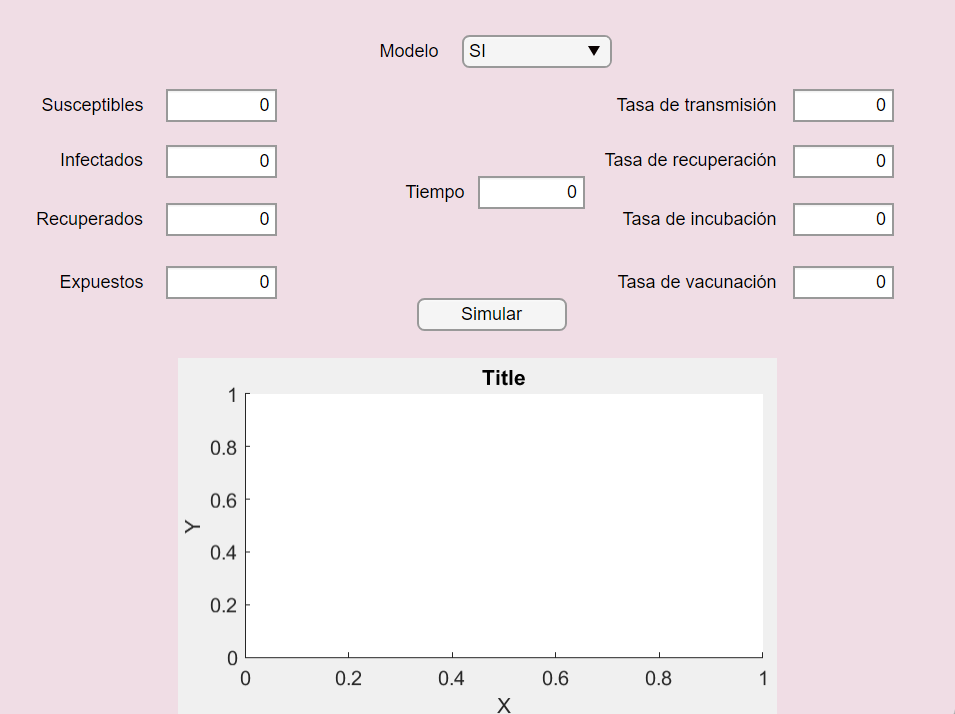
\includegraphics[width=0.7\textwidth]{img/inicio app.png}
        \caption{Interfaz inicial de la aplicación}
        \label{fig:app inicio}
        \vspace{0.5cm} % Ajusta el espacio vertical entre la imagen y el texto
    \end{figure}

Desde el menú desplegable superior se puede seleccionar el modelo deseado entre SI, SIS, SIR, SEIR. A continuación, el usuario puede introducir los valores iniciales para cada grupo de población:
\begin{itemize}
    \item Susceptibles
    \item Infectados
    \item Recuperados
    \item Expuestos
\end{itemize}
Así como las tasas características del modelo:
\begin{itemize}
    \item Tasa de transmisión
    \item Tasa de recuperación
    \item Tasa de incubación
    \item Tasa de vacunación
\end{itemize}
También se introduce el tiempo de simulación total (en días o unidades temporales equivalentes). Una vez completados los parámetros, el botón "Simular" permite ejecutar la simulación. Los resultados se visualizan automáticamente en una gráfica situada en la parte inferior.

Esta interfaz facilita el análisis comparativo entre modelos y permite observar el comportamiento dinámico del sistema epidemiológico en función de las distintas condiciones iniciales.

\subsection{Selección del modelo}

La aplicación permite seleccionar el tipo de modelo epidemiológico a simular mediante un menú desplegable ubicado en la parte superior central de la interfaz. Los modelos disponibles son:

\begin{itemize}
    \item \textbf{SI}: modelo simple de contagio sin recuperación.
    \item \textbf{SIS}: permite reinfección tras la recuperación.
    \item \textbf{SIR}: incluye inmunidad permanente tras la recuperación.
    \item \textbf{SEIR}: añade una fase de exposición previa al contagio.
    \item \textbf{SIRV}: añade una tasa de vacunación al modelo SIR.
    \item \textbf{SEIRV}: añade tasa de vacunación al modelo SEIR.
\end{itemize}

Al seleccionar un modelo, la interfaz se adapta automáticamente, activando o desactivando los campos de entrada correspondientes. Por ejemplo, el campo “Expuestos” sólo se habilita si se selecciona el modelo SEIR, y la “Tasa de vacunación” se emplea únicamente en aquellos modelos que incorporan estrategias de vacunación como SIRV o SEIRV. Además al seleccionar un modelo, se cargan automáticamente valores por defecto en todos los parámetros y campos de entrada. Esto permite ejecutar simulaciones de ejemplo directamente, sin necesidad de introducir manualmente todos los datos. Estos valores predefinidos están pensados para ofrecer resultados representativos del comportamiento típico de cada modelo.


\subsection{Ejecución de simulaciones}

Una vez configurados los valores iniciales de la población y los parámetros del modelo, el usuario debe presionar el botón \textbf{Simular}. Al hacerlo, se ejecuta la resolución del sistema de ecuaciones diferenciales asociado al modelo epidemiológico. Las simulaciones se realizan empleando funciones de MATLAB basadas en ode45, y los resultados se visualizan directamente en el eje gráfico de la interfaz. Las curvas generadas permiten analizar el comportamiento de cada grupo poblacional en el tiempo.

El sistema también incluye controles para reiniciar los parámetros y ejecutar nuevas simulaciones con diferentes configuraciones.

\subsection{Casos de uso prácticos}

A continuación, se presentan dos ejemplos prácticos de uso de la aplicación, explicados paso a paso. Estos permiten comprobar cómo se comporta la simulación en diferentes escenarios epidemiológicos.

\vspace{1em}
\subsubsection{Ejemplo 1 – Simulación con modelo SIR}

\textbf{Pasos:}
\begin{enumerate}
    \item Seleccionar el modelo \textbf{SIR} en el menú desplegable \ref{fig:eleccion sir}.
     \item Verificar que los valores por defecto se han cargado correctamente (se pueden modificar si se desea)\ref{fig:datos defecto}.
      \item Pulsar el botón \textbf{Simular}.

     
    \item Observar la evolución temporal de las tres poblaciones en la gráfica \ref{fig:simulacion sir ap}
    \begin{figure}[H]
        \centering
        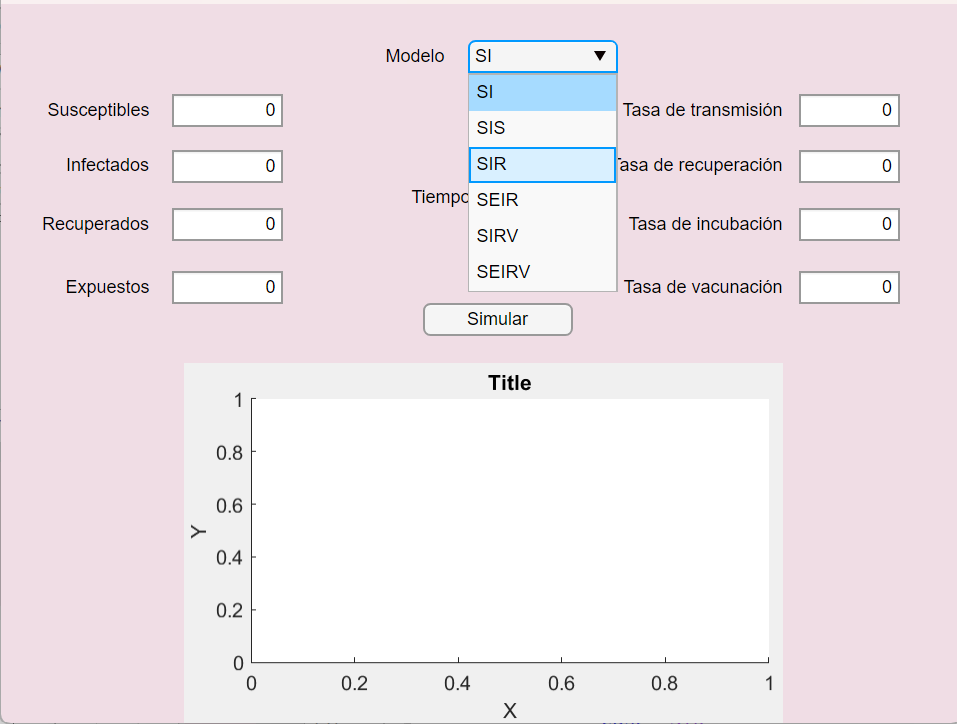
\includegraphics[width=0.7\textwidth]{img/eleccion modelo SIR.png}
        \caption{Elección del modelo, en est caso SIR}
        \label{fig:eleccion sir}
        \vspace{0.5cm} % Ajusta el espacio vertical entre la imagen y el texto
    \end{figure}
   

    \begin{figure}[H]
        \centering
        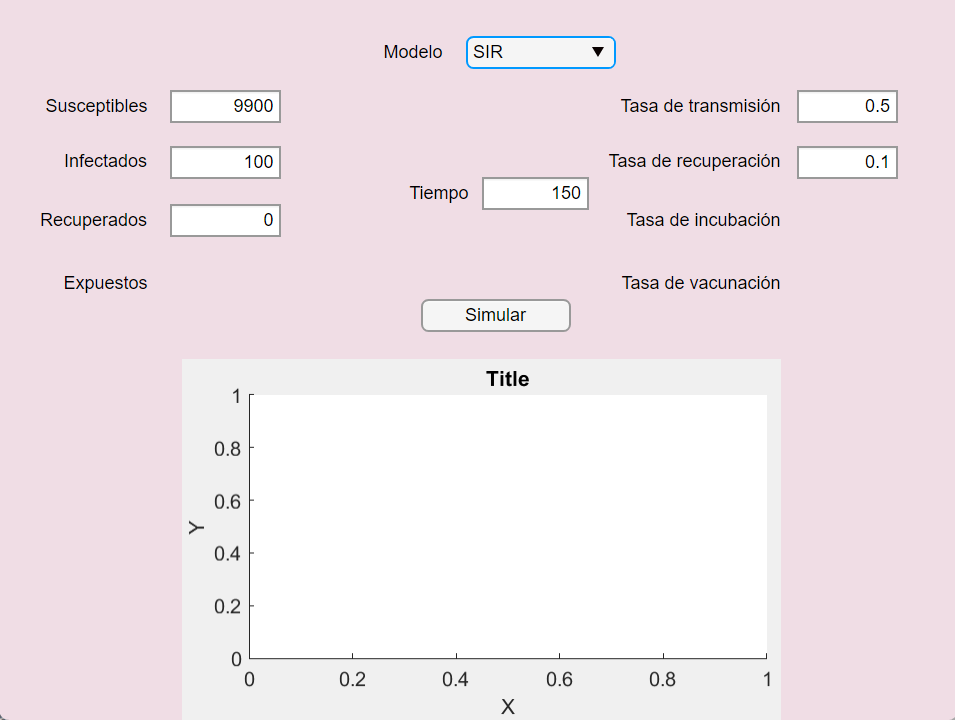
\includegraphics[width=0.7\textwidth]{img/modelo sir datos.png}
        \caption{Comprobación de que salen los datos por defecto}
        \label{fig:datos defecto}
        \vspace{0.5cm} % Ajusta el espacio vertical entre la imagen y el texto
    \end{figure}
   
   
    \begin{figure}[H]
        \centering
        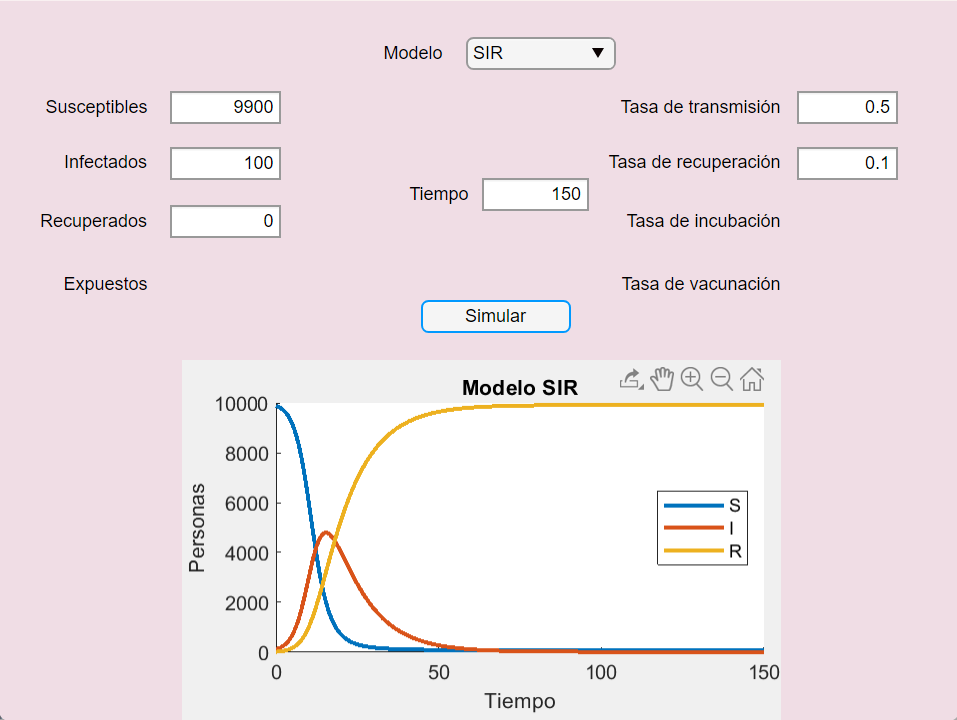
\includegraphics[width=0.7\textwidth]{img/simulacion sir app.png}
        \caption{Simulación del modelo SIR en la aplicación}
        \label{fig:simulacion sir ap}
        \vspace{0.5cm} % Ajusta el espacio vertical entre la imagen y el texto
    \end{figure}
\end{enumerate}

Este ejemplo permite visualizar cómo aumenta inicialmente el número de infectados, hasta alcanzar un pico, seguido de una disminución conforme los individuos se recuperan y se inmunizan.

\vspace{1em}
\subsubsection{Ejemplo 2 – Simulación con modelo SEIR}

\textbf{Se siguien los mismos pasos que antes:}
\begin{enumerate}
    \item Seleccionar el modelo \textbf{SEIR} \ref{fig:eleccion seirv}.
    \item Comprobar que los valores se han precargado automáticamente, se pueden cambiar si se desea.
    \item Hacer clic en \textbf{Simular}.
    \item Observar el efecto del regulador PID: el número de infectados se mantiene bajo control y disminuye más rápidamente \ref{fig:eseeir}.
\end{enumerate}

\begin{figure}[H]
        \centering
        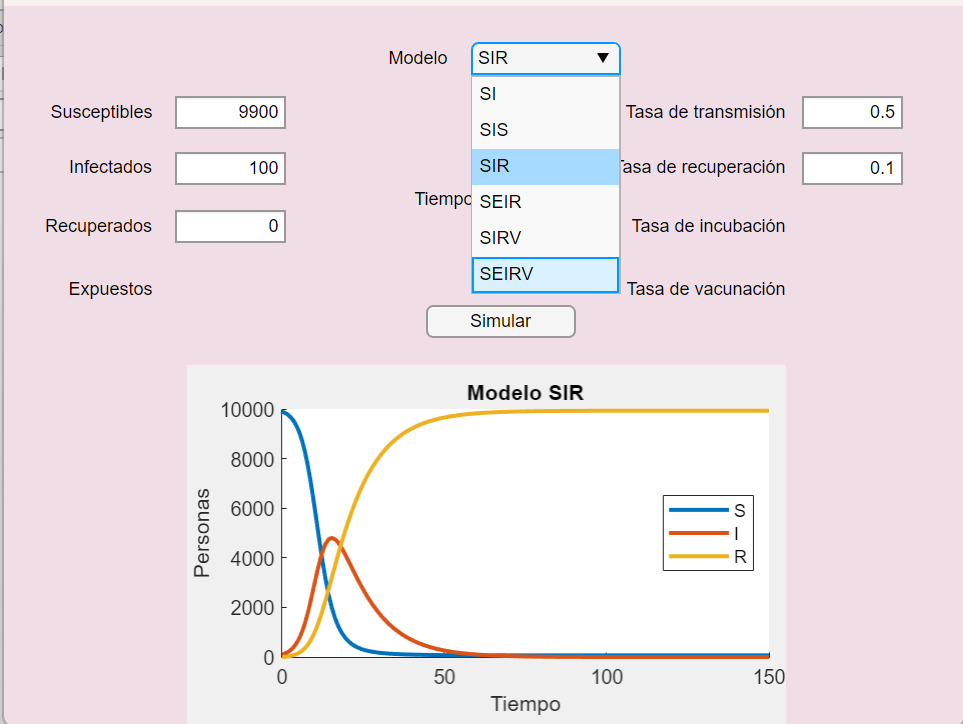
\includegraphics[width=0.7\textwidth]{img/eleccion SEIR.png}
        \caption{Elección del modelo, en este caso SEIRV}
        \label{fig:eleccion seirv}
        \vspace{0.5cm} % Ajusta el espacio vertical entre la imagen y el texto
    \end{figure}


\begin{figure}[H]
        \centering
        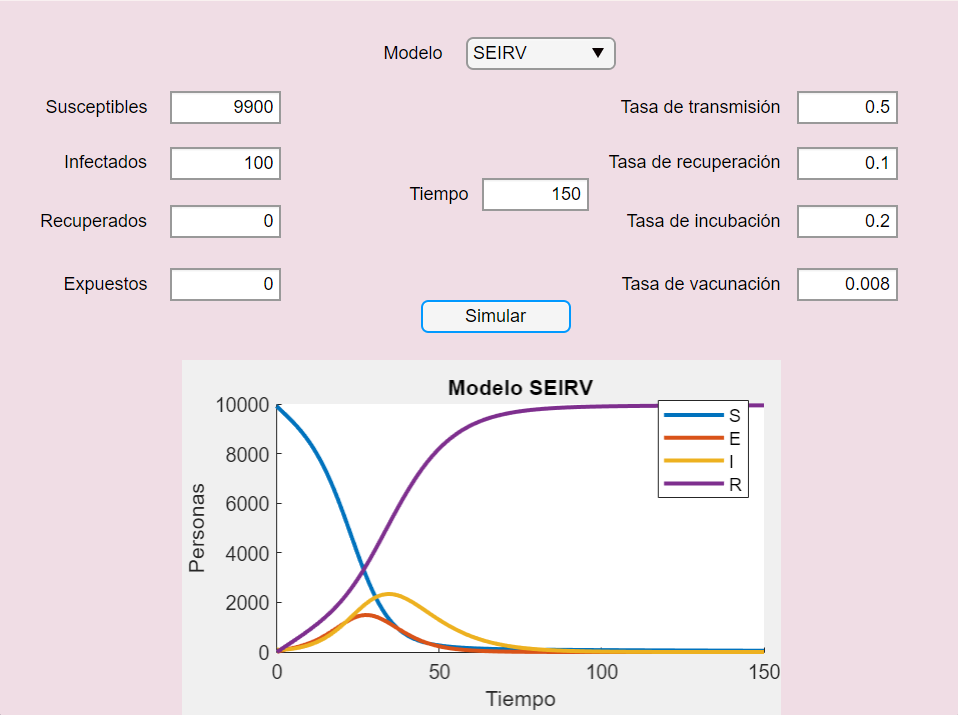
\includegraphics[width=0.7\textwidth]{img/simulacion.png}
        \caption{Simulación del modelo SEIRV en la aplicación con los datos predefinidos}
        \label{fig:eseeir}
        \vspace{0.5cm} % Ajusta el espacio vertical entre la imagen y el texto
    \end{figure}










\apendice{Manual del investigador}

\section{Estructura de directorios}
A continuación se describe la estructura del proyecto, así como el contenido y propósito de cada carpeta y archivo relevante, todo está en el repositorio de GitHub. El proyecto está organizado en una estructura de carpetas que separa claramente los distintos componentes como se describe a continuación.

\begin{itemize}
    \item \textbf{Carpeta \texttt{aplicación}} \\

Contiene los archivos necesarios para la ejecución y distribución de la aplicación desarrollada en \textit{App Designer} de MATLAB. A continuación, se describen los elementos incluidos:

\begin{itemize}
    \item \texttt{aplicacion\_modelos.mlapp}: archivo principal de la aplicación, editable y ejecutable desde MATLAB con App Designer.
    
    \item \texttt{aplicacion\_modelos.exe}: versión compilada de la aplicación para ejecutarse de forma autónoma sin necesidad de abrir MATLAB.
    
    \item \texttt{MyAppInstaller\_web.exe}: instalador web proporcionado por MATLAB que permite instalar las dependencias necesarias para ejecutar la aplicación si el usuario no dispone de una instalación completa de MATLAB.
    
    \item Carpeta \texttt{aplicacion\_modelos}: contiene los archivos auxiliares generados tras la compilación de la aplicación. Son necesarios para su correcto funcionamiento sin entorno MATLAB.
    
    \item \texttt{README.txt}: archivo de texto que actúa como guía de usuario. Describe los componentes anteriores y cómo instalar y ejecutar la aplicación.
\end{itemize}


    \item \textbf{Carpeta bibliografía} \\
    Documentos y artículos científicos en .pdf utilizados para entender y fundamentar los modelos epidemiológicos.

    \item \textbf{Carpeta documentación overleaf} \\
    Carpeta que contiene los archivos fuente del TFG escritos en LaTeX:
    \begin{itemize}
        \item \texttt{Carpeta img}: imágenes utilizadas en la memoria y anexos.
        \item \texttt{Carpeta tex}: secciones y capítulos del TFG, tanto memoria como anexos.
        \item \texttt{anexos.tex, memoria.tex}: documentos principales del trabajo.
        \item \texttt{bibliografia.bib, bibliografiaAnexos.bib}: bases de datos bibliográficas en formato BibTeX.
    \end{itemize}

    \item \textbf{Carpeta informes entrega} \\
    Archivos PDF del trabajo final entregado:
    \begin{itemize}
        \item \texttt{anexos\_Lucía\_Segura.pdf}: anexos en formato .pdf.
        \item \texttt{memoria\_Lucía\_Segura.pdf}: memoria en formato .pdf.
    \end{itemize}

    \item \textbf{Carpeta MATLAB} \\
    Archivos y resultados de las simulaciones en entorno MATLAB:
    \begin{itemize}
        \item \texttt{/resultados/}: gráficas generadas desde scripts.
        \item \texttt{modelo\_SIR\_PID.m}: código de simulación del modelo SIR con control PID.
        \item Imágenes del controlador y parámetros PID.
    \end{itemize}

    \item \textbf{Carpeta Simulink} \\
    Contiene los modelos diseñados en Simulink y sus resultados visuales:
    \begin{itemize}
        \item \texttt{Carpeta modelos Simulink}: archivos \texttt{.slx} de los modelos SI, SIS, SIR, SEIR, SIRV y SEIRV.
        \item \texttt{carpeta Otras simulaciones}: contiene capturas de pantalla y gráficos generados al modificar distintos parámetros en los modelos matemáticos. Estas simulaciones adicionales permiten realizar un análisis comparativo entre diferentes escenarios y evaluar la sensibilidad del modelo ante variaciones en sus condiciones iniciales o parámetros clave.
        \item \texttt{Carpeta resultados}: imágenes de resultados (\texttt{.jpg}).
        \item Imágenes de los diagramas (\texttt{.png}).
    \end{itemize}

    \item README.md \\
    Archivo de introducción al proyecto, útil para usuarios que lo descarguen por primera vez.
\end{itemize}

Esta organización permite acceder rápidamente a cada componente del proyecto según su función: código, documentación, simulaciones o entregas finales.


\section{Compilación, instalación y ejecución del proyecto}

El proceso completo de instalación del entorno \textit{MATLAB} y la ejecución de la aplicación se encuentra detallado en el Apéndice B, concretamente en el apartado B.2. A continuación, se resumen las consideraciones técnicas más relevantes desde el punto de vista del desarrollo y la distribución del software.

El proyecto ha sido desarrollado en \textbf{MATLAB R2019b}, por lo que se recomienda utilizar esta misma versión o una superior compatible con los archivos generados.

\subsection*{Requisitos del entorno de desarrollo}
Para ejecutar los modelos y la aplicación, se requiere disponer de los siguientes componentes instalados:

\begin{itemize}
    \item \textbf{MATLAB} (versión R2019b o superior)
    \item \textbf{Simulink}
    \item \textbf{Control System Toolbox}
    \item \textbf{App Designer}
\end{itemize}

Los modelos matemáticos implementados en Simulink se encuentran en la carpeta \texttt{/Simulink/modelos\_Simulink/} con extensión \texttt{.slx}, y pueden abrirse directamente desde el entorno MATLAB. Por su parte, los scripts, incluyendo el controlador PID desarrollado sobre el modelo SIR, están ubicados en la carpeta \texttt{/MATLAB/} con extensión \texttt{.m}.

La aplicación desarrollada con App Designer se encuentra en la carpeta \texttt{/aplicación/}, dentro del archivo \texttt{aplicacion\_modelos.mlapp}.

\subsection*{Ejecución de la aplicación}

La carpeta \texttt{aplicación} contiene todos los archivos necesarios para ejecutar la \textbf{Aplicación de Modelos Epidemiológicos}. Existen dos modos de ejecución, en función de si el usuario dispone de MATLAB instalado o no:

\begin{enumerate}
    \item \textbf{Con MATLAB instalado}: utilizando directamente el archivo \texttt{.mlapp}.
    \item \textbf{Sin MATLAB instalado}: mediante el ejecutable compilado \texttt{.exe} y el instalador de runtimes de MATLAB.
\end{enumerate}

\subsection*{Archivos incluidos en la carpeta \texttt{aplicación}}

\begin{itemize}
    \item \texttt{aplicacion\_modelos.mlapp}: interfaz gráfica de usuario desarrollada con App Designer. Ejecutable desde MATLAB.
    
    \item \texttt{aplicacion\_modelos.exe}: versión compilada de la aplicación para sistemas Windows (64 bits). Ejecutable independiente que requiere los runtimes de MATLAB.

    \item \texttt{MyAppInstaller\_web.exe}: instalador automático de los \textit{MATLAB Runtime} (MCR), necesarios para ejecutar el archivo \texttt{.exe} si no se dispone de MATLAB instalado.

    \item Carpeta \texttt{aplicacion\_modelos/}: contiene los archivos auxiliares generados durante la compilación de la aplicación.

    \item \texttt{README.txt}: archivo de texto con instrucciones detalladas sobre instalación, ejecución y requisitos del sistema.
\end{itemize}

\subsection*{Requisitos del sistema}

\begin{itemize}
    \item \textbf{Con MATLAB instalado:}
    \begin{itemize}
        \item MATLAB R2019b (o superior)
        \item App Designer
        \item No requiere instalar runtimes adicionales
    \end{itemize}

    \item \textbf{Sin MATLAB instalado:}
    \begin{itemize}
        \item Sistema operativo Windows 64 bits
        \item Espacio libre en disco: mínimo 500 MB
        \item Instalación de runtimes mediante \texttt{MyAppInstaller\_web.exe}
    \end{itemize}
\end{itemize}

\subsection*{Instrucciones de instalación y ejecución}

\begin{itemize}
    \item \textbf{Opción 1: Ejecución con MATLAB}
    \begin{enumerate}
        \raggedright
        \item Abrir MATLAB.
        \item Acceder al directorio donde se encuentra el archivo \texttt{aplicacion\_modelos.mlapp}.
        \item En la línea de comandos de MATLAB, ejecutar: \texttt{\textgreater{}\textgreater{} open('aplicacion\_modelos.mlapp')}.
        \item Pulsar en el botón “Run” dentro de App Designer.
        \item La aplicación se iniciará y permitirá interactuar con los modelos epidemiológicos.
    \end{enumerate}

    \item \textbf{Opción 2: Ejecución sin MATLAB}
    \begin{enumerate}
        \item Instalar los runtimes de MATLAB:
        \begin{itemize}
            \item Ejecutar \texttt{MyAppInstaller\_web.exe}.
            \item Seguir los pasos del asistente de instalación.
        \end{itemize}
        \item Ejecutar la aplicación compilada:
        \begin{itemize}
            \item Hacer doble clic en \texttt{aplicacion\_modelos.exe}.
            \item La aplicación se iniciará automáticamente.
        \end{itemize}
    \end{enumerate}
\end{itemize}

\subsection*{Notas adicionales}

\begin{itemize}
    \item Si ya se dispone de MATLAB instalado, no es necesario ejecutar \texttt{MyAppInstaller\_web.exe} ni utilizar la versión compilada.
    \item La instalación de los runtimes puede tardar varios minutos dependiendo de la velocidad de conexión y del sistema.
    \item La desinstalación de los MATLAB Runtime puede realizarse desde el Panel de control de Windows → “Programas y características” → “MATLAB Runtime”.
\end{itemize}



\section{Pruebas del sistema}
Durante el desarrollo del proyecto se llevaron a cabo diferentes pruebas para asegurar el correcto funcionamiento de los modelos implementados y de la interfaz gráfica desarrollada:

\begin{itemize}
    \item Se validó que los modelos epidemiológicos (SI, SIS, SIR, SEIR y SIR con control PID) producen resultados coherentes para diferentes combinaciones de parámetros.

    \item En los modelos SIR y SEIR se añadió un componente de \textbf{vacunación}. Se realizaron pruebas con tasas de vacunación constantes, observando cómo influye en la evolución de los individuos. Como resultado, se observaron curvas más planas o reducción del pico epidémico, en línea con lo esperado teóricamente.

    \item Se ejecutaron simulaciones con \textbf{datos reales de enfermedades infecciosas} contrastando los resultados generados por el modelo con los datos empíricos, para verificar la validez de la estructura matemática.

    \item Se realizaron pruebas específicas con el modelo \textbf{SIR regulado mediante un controlador PID}, comprobando que el sistema responde adecuadamente a variaciones en el número de infectados y que el regulador permite mitigar oscilaciones o picos no deseados.

    \item En cuanto a la aplicación gráfica (.mlapp) se verificó que cada modelo se carga correctamente, que los valores por defecto permiten una simulación directa y que la visualización gráfica es coherente con la salida del modelo.

    
\end{itemize}

Estas pruebas confirman la robustez funcional del sistema, tanto desde el punto de vista técnico como de su aplicabilidad para visualizar dinámicas epidemiológicas complejas.

\section{Instrucciones para la modificación o mejora del proyecto}

El proyecto ha sido desarrollado de forma modular, por lo que resulta relativamente sencillo introducir mejoras. A continuación, se describen algunas recomendaciones para su modificación o ampliación:

\begin{itemize}
    \item \textbf{Ampliación de modelos:} Se pueden implementar nuevos modelos epidemiológicos (por ejemplo, SEIRS, modelos estocásticos o con movilidad) reutilizando la estructura existente en la aplicación.

    \item \textbf{Incorporación de nuevas funcionalidades:} Sería interesante añadir funciones como el cálculo automático del número básico de reproducción \( R_0 \), análisis de sensibilidad, o exportación de resultados en CSV o PDF.

    \item \textbf{Mejora de la interfaz:} La interfaz puede ampliarse con pestañas o menús desplegables para facilitar la navegación. También se podría implementar la carga de datos desde archivos externos.

    \item \textbf{Uso de datos reales actualizados:} El proyecto puede conectarse con fuentes de datos abiertas (como la OMS o Our World in Data) para actualizar automáticamente los valores utilizados en las simulaciones.


\end{itemize}

Estas sugerencias pueden servir de base para futuras mejoras, tanto a nivel técnico como funcional.





\apendice{Descripción de aquisición y tratamiento de datos}

\section{Descripción formal de los datos}
Los datos utilizados en este trabajo han sido extraídos de diversos estudios científicos y publicaciones especializadas, todos ellos debidamente citados en la bibliografía de la memoria. No se han empleado conjuntos de datos descargables o bases oficiales, sino que los valores han sido recogidos manualmente o digitalizados a partir de tablas y gráficas publicadas en dichos estudios.

Los datos empleados incluyen:
\begin{itemize}
    \item Número de personas infectadas, susceptibles, recuperadas y población total.
    \item Parámetros epidemiológicos clave:
        \begin{itemize}
            \item Tasa de transmisión (\( \beta \))
            \item Tiempo medio de recuperación (\( \gamma^{-1} \))
            \item Tiempo medio de incubación (en modelo SEIR)
            \item Cobertura de vacunación.
            \item Número reproductivo básico (\( R_0 \)).
        \end{itemize}
\end{itemize}

En algunos casos, los parámetros han sido directamente obtenidos de los estudios. En otros, han sido estimados o deducidos a partir de las relaciones matemáticas de los modelos, como por ejemplo:

\[
R_0 = \frac{\beta}{\gamma}
\quad \text{o} \quad
\beta = R_0 \cdot \gamma
\]

\bigskip
Los datos han sido tratados en MATLAB para ajustarlos al formato de entrada de los modelos. 
Estos datos han servido tanto para calibrar los modelos (SI, SIR, SEIR con y sin vacunación) como para comparar los resultados simulados con los patrones observados en situaciones reales.




\section{Descripción clínica de los datos}

Desde un punto de vista clínico, los datos empleados reflejan la evolución temporal de una enfermedad infecciosa en una población concreta, segmentada en distintos estados epidemiológicos:

\begin{itemize}
    \item \textbf{Susceptibles (S):} individuos sanos sin inmunidad previa, que pueden infectarse al entrar en contacto con agentes infecciosos. Clínicamente, representan la población en riesgo de contraer la enfermedad.
    \item \textbf{Expuestos (E):} personas que han sido infectadas recientemente y que se encuentran en un período de incubación durante el cual aún no son contagiosas. Clínicamente, este grupo representa la fase pre-sintomática o latente de la infección.
    \item \textbf{Infectados (I):} individuos que actualmente tienen el virus y son capaces de transmitirlo a los susceptibles. Este grupo clínico puede incluir desde casos asintomáticos hasta pacientes con síntomas severos.
    \item \textbf{Recuperados (R):} se agrupan tanto los individuos que han superado la infección y desarrollado inmunidad, como aquellos que han adquirido protección a través de la vacunación. En ambos casos, se asume que ya no pueden infectarse ni transmitir la enfermedad.
\end{itemize}

También es importante hacer una descripción clínica de las principales tasas epidemiológicas que se utilizan en este estudio.


\begin{itemize}
    \item \textbf{Tasa de transmisión, $\beta$:} Representa la probabilidad o velocidad con la que una persona susceptible se infecta al entrar en contacto con un individuo infectado. Clínicamente, esta tasa está influenciada por la virulencia del patógeno, el comportamiento social (contactos, movilidad), y medidas de prevención (uso de mascarillas, higiene, distanciamiento social). Un aumento en $\beta$ puede indicar mayor contagiosidad o relajación de medidas sanitarias.
    \item \textbf{Tasa de incubación, $\sigma$:} indica la velocidad con la que los individuos en el estado expuesto (infectados pero no contagiosos) pasan a ser infectantes. Clínicamente, esta tasa está relacionada con el período de incubación del virus, es decir, el tiempo que tarda en manifestarse la capacidad de contagiar tras la infección.
    \item \textbf{Tasa de recuperación, $\gamma$:} refleja la velocidad con la que los infectados superan la enfermedad y pasan al estado de recuperados, asumiendo inmunidad. Clínicamente, esta tasa depende de la duración media de la enfermedad y del acceso a tratamientos médicos eficaces. Un aumento en $\gamma$ puede indicar mejoras en la atención sanitaria o en la respuesta inmune.
    \item \textbf{Tasa de vacunación, $\nu$}: representa la velocidad a la que los individuos susceptibles reciben la vacuna y adquieren inmunidad. Clínicamente, esta tasa refleja la capacidad y cobertura de vacunación en la población, afectando directamente al tamaño del grupo susceptible y, por tanto, al control de la epidemia.
    
\end{itemize}

Esta descripción clínica de las variables y parámetros permite entender cómo se traduce la información epidemiológica en las ecuaciones del modelo, y facilita la interpretación de los resultados para la toma de decisiones sanitarias.

\section{Datos utilizados}
A continuación, se describen los datos utilizados para cada modelo, incluyendo su origen, características y el procedimiento seguido para su obtención y tratamiento.

\subsection{Modelo SI}
Se va a estudiar la enfermedad en la región MENA\footnote{Oriente Medio y Norte de África.}, cuya población total se estima en aproximadamente 400 millones de personas. En cuanto a las personas infectadas con VIH es de alrededor de 240000 personas \cite{Khorrami2023}.

La tasa de transmisión es de 0,105 \cite{shakiba2021epidemiological} para esta enfermedad. Sin embargo, para utilizarlo correctamente es necesario ajustar la beta, para facilitar las ecuaciones no se ha metido la población total, por eso hay que ajustar beta como se muestra en la ecuación \eqref{eq:beta_efectiva2}.
\begin{equation}
\beta_{\text{efectiva}} = \frac{\beta}{N} = \frac{0.105}{400\,000\,000} = 2.625 \times 10^{-10}
\label{eq:beta_efectiva2}
\end{equation}

\subsection{Modelo SIS}
Se ha tomado como referencia la situación epidemiológica en Estados Unidos durante el 2019. En ese año, la población total del país era aproximadamente 328 millones de personas, en cuanto a los casos de personas infectadas ascendía a 1603473 personas \cite{pollock2023estimated}.

La tasa de la enfermedad pude variar en función del comportamiento social, el uso de métodos de protección y otros factores. Pero para este estudio se ha estimado una tasa de 0.25, hay que calcular la beta efectiva \eqref{eq:beta_efectiva}.
\begin{equation}
\beta_{\text{efectiva}} = \frac{\beta}{N} = \frac{0.25}{328\,000\,000} = 7 \times 10^{-10}
\label{eq:beta_efectiva}
\end{equation}


Respecto a la tasa de recuperación, se considera que, en un país con un sistema sanitario desarrollado como Estados Unidos, los individuos infectados reciben tratamiento de forma relativamente rápida. Aunque sin tratamiento la infección puede durar semanas o incluso meses, con tratamiento, el tiempo medio de recuperación se estima en unos 7 días. Por lo tanto, la tasa de recuperación se calcula como se oberva en \eqref{eq:gamma}.

\begin{equation}
\gamma = \frac{1}{\text{tiempo de recuperación}} = \frac{1}{7}
\label{eq:gamma}
\end{equation}


\subsection{Modelo SIR}
Se ha elegido analizar la propagación del sarampión en Estados Unidos antes de la introducción de la vacuna en 1963. El país contaba con una población de aproximadamente 189 millones de personas \cite{datosmacro_usa_1963}, mientras que se registraban alrededor de 500 mil casos anuales. Datos que reflejan la alta incidencia del sarampión.
Uno de los parámetros más relevantes para modelar esta enfermedad es el número básico de reproducción, que representa el número medio de personas susceptibles que puede llegar a contagiar un solo individuo infectado en una población completamente susceptible. En el caso del sarampión, este valor es excepcionalmente alto, estimándose en torno a $R_0$ = 12 \cite{solomon2019peter}. Significa que, en ausencia de medidas de control, cada persona infectada podría contagiar a doce individuos, lo que explica su elevada transmisibilidad y su capacidad para provocar grandes brotes epidémicos.

Además, se conoce que el tiempo de recuperación de la enfermedad es de 14 días \cite{ops_sarampion}. Esto implica que la tasa de recuperación (~$\gamma$) se calcula en la ecuación \eqref{eq:gamma_14}
\begin{equation}
\gamma = \frac{1}{\text{tiempo medio de recuperación}} = \frac{1}{14} = 0{,}071 \,\text{días}^{-1}
\label{eq:gamma_14}
\end{equation}

Dado que la relación entre $R_0$, beta y gamma viene dada por la fórmula \eqref{eq:R0}
\begin{equation}
R_0 = \frac{\beta}{\gamma}
\label{eq:R0}
\end{equation}

Se despeja beta para poder calcular la tasa de transmisión \eqref{eq:beta_calculo}
\begin{equation}
\beta = R_0 \times \gamma = 12 \times 0{,}071 = 0{,}852
\label{eq:beta_calculo}
\end{equation}

Una vez se ha calculado beta\eqref{eq:beta_calculo}, hay que calcular la beta ajustada para este modelo, es decir, la beta efectiva \eqref{eq:beta_efectiva2}
\begin{equation}
\beta_{\text{efectiva}} = \frac{\beta}{N} = \frac{0{,}852}{189\,000\,000} = 4{,}5 \times 10^{-9}
\label{eq:beta_efectiva2}
\end{equation}

\subsection{Modelo SIRV}
La única diferencia introducida es la incorporación de una tasa de vacunación correspondiente a una cobertura del 92,7\% de la población en un periodo de seis meses, lo cual se ajusta a datos reales observados en campañas de vacunación contra el sarampión. Este porcentaje se ha convertido en un valor de tasa ($\nu$) para integrarlo dentro del sistema de ecuaciones del modelo SIRV, y así simular cómo evolucionaría la epidemia bajo una estrategia de inmunización masiva \cite{cdc_measles_cases_2025}.

De esta manera, se busca evaluar cuantitativamente cómo la vacunación modifica la evolución del brote, en particular en términos de reducción de contagios y aceleración de la inmunidad colectiva, y contrastar estos resultados con los obtenidos previamente en ausencia de intervenciones.
Se tiene la cobertura de vacunación, pero hay que calcular la tasa de vacunación con los datos que se han obtenido. Se calcula a partir de la siguiente fórmula \eqref{eq:nu_vacunacion}. 
\begin{equation}
\nu = \frac{-\ln(1 - 0{,}927)}{183} \approx 0{,}014
\label{eq:nu_vacunacion}
\end{equation}
Esto significa que aproximadamente el 1,4\% de la población susceptible se vacuna cada día durante ese periodo, adquiriendo inmunidad y pasando directamente al compartimento de recuperados. Esta tasa se incorpora en el modelo como un nuevo flujo desde susceptibles a recuperados, simulando el efecto de la vacunación masiva sobre la dinámica de propagación del sarampión.






\subsection{Modelo SEIR}
Se ha elegido como caso de estudio la evolución de la COVID-19 en España, desde la aparición del primer caso confirmado, registrado el 31 de enero de 2020 \cite{primer_caso_covid_espana}. Desde esa fecha hasta el 28 de diciembre de 2020 a las 14:00 horas, se notificaron oficialmente un total de 1879413 casos acumulados de personas infectadas por SARS-CoV-2 \cite{sanidad_covid_situacion}. En ese mismo año, la población total de España era de aproximadamente 47370000 habitantes \cite{datacommons_espana_demografia}.

En las primeras fases de la pandemia, el número básico de reproducción del virus SARS-CoV-2 se situaba, según estimaciones epidemiológicas, entre 2 y 3 \cite{garcia_r0_desescalada}. Esto indica que cada persona infectada transmitía el virus entre 2 y 3 personas, lo que implica una tendencia clara al crecimiento exponencial del brote en ausencia de medidas de control o inmunidad previa en la población.

En cuanto a los parámetros clínicos de la enfermedad, el periodo de incubación, entendido como el intervalo desde la exposición al virus hasta el momento en que el individuo se vuelve contagioso, se estima con una media de 5.4 días \cite{lauer2020incubation}. Hay que calcular la tasa de incubación ($\sigma$)\eqref{eq:sigma}
\begin{equation}
\sigma = \frac{1}{\text{tiempo de incubación}} = \frac{1}{5{,}4} = 0{,}185
\label{eq:sigma}
\end{equation}

Por otro lado, el tiempo medio de recuperación depende de la gravedad del cuadro clínico. En los casos leves, suele rondar las 2 semanas, mientras que en los casos moderados o graves puede extenderse entre 3 y 6 semanas. Para simplificar el análisis y mantener la coherencia en el modelo, se considerará un tiempo medio de recuperación de 14 días \cite{ada_duracion_covid}. Hay que calcular la tasa de recuperación \eqref{eq:gamma_7}
\begin{equation}
\gamma = \frac{1}{\text{tiempo medio de recuperación}} = \frac{1}{14} = 0{,}071 \,\text{días}^{-1}
\label{eq:gamma_7}
\end{equation}

Para finalizar, hay que calcular la tasa de transmisión, para ello utilizamos el $R_0$, ya que relaciona la gamma y beta. Se aplica la fórmula del $R_0$. Se va a optar por utilizar el valor de $R_0$ = 3, ya que es un escenario más desfavorable y representativo, es más contagioso. La ecuacion \eqref{eq:R0} se utiliza para calcular beta.\eqref{eq:beta_R0_gamma}
\begin{equation}
\beta = R_0 \times \gamma = 3 \times 0{,}071 = 0{,}213
\label{eq:beta_R0_gamma}
\end{equation}

Una vez se ha calculado la beta, hay que calcular la beta efectiva\eqref{eq:beta_efectiva_final}.
\begin{equation}
\beta_{\text{efectiva}} = \frac{\beta}{N} = \frac{0{,}213}{47\,370\,000} \approx 4{,}5 \times 10^{-9}
\label{eq:beta_efectiva_final}
\end{equation}



\subsection{Modelo SEIRV}
Con el fin de ampliar el análisis realizado sobre el COVID-19 mediante el modelo SEIR, se ha decidido incorporar la vacunación en la simulación a través del modelo SEIRV. Permite estudiar cómo una campaña de vacunación influye en la dinámica de propagación del virus, proporcionando una visión más realista del contexto epidemiológico vivido en España durante la pandemia.
Para mantener la coherencia entre escenarios, se han conservado los mismos parámetros epidemiológicos utilizados en el modelo SEIR básico: la tasa de transmisión, el tiempo de incubación y la tasa de recuperación. La diferencia es la inclusión de un parámetro, la tasa de vacunación, que representa el efecto de la inmunización masiva iniciada en España a finales de 2020.
Según los datos oficiales, la campaña de vacunación comenzó el 27 de diciembre de 2020, y hasta el 15 de enero de 2021 se habían administrado 768.950 dosis \cite{sanidad_giv_20210115}. Posteriormente, la cobertura vacunal alcanzó el 92,6\% de la población en un año \cite{sanidad_historico_covid}. Para incorporar esta información en el modelo, es necesario calcular la tasa diaria de vacunación, lo cual se realiza con la siguiente fórmula \eqref{eq:nu_926}.
\begin{equation}
\nu = \frac{-\ln(1 - 0{,}926)}{365} \approx 0{,}0071
\label{eq:nu_926}
\end{equation}

Este valor indica que aproximadamente el 0,71\% de la población susceptible se vacuna cada día durante ese periodo. En el modelo, estas personas abandonan directamente el compartimento de susceptibles y pasan al de recuperados, ya que se considera que la vacunación confiere una inmunidad funcional equivalente a la adquirida tras superar la infección.
Se mantiene, la misma estructura conceptual del modelo SEIR. La única diferencia es la inclusión del flujo adicional introducido por la vacunación. Así, el modelo SEIRV permite simular con mayor precisión cómo las campañas de inmunización modifican la evolución de la pandemia, en particular reduciendo el número de contagios y acelerando el logro de la inmunidad colectiva.



\section{Información relevante de los simulaciones}

Las simulaciones realizadas permiten analizar la evolución temporal de la epidemia bajo distintos escenarios y condiciones iniciales. A través de estas simulaciones se observan dinámicas clave de la propagación del virus, lo que facilita la evaluación de posibles estrategias de control.

 Variaciones en parámetros fundamentales, provocan cambios significativos tanto en la magnitud del brote como en su duración. Por ejemplo, un incremento en la tasa de vacunación reduce notablemente el número máximo de infectados y acorta el tiempo total de propagación de la epidemia. La curva de infectados presenta un pico cuya altura y momento dependen directamente de los parámetros epidemiológicos y de las intervenciones aplicadas.
Estas simulaciones permiten identificar puntos críticos a partir de los cuales es posible controlar o incluso erradicar la epidemia mediante intervenciones adecuadas. Los resultados obtenidos aportan una visión cuantitativa del comportamiento dinámico del sistema epidemiológico, lo que resulta útil para diseñar estrategias de mitigación que minimicen el impacto sanitario.

No obstante, es importante tener en cuenta que el modelo se basa en una serie de supuestos que simplifican la realidad para hacer el sistema tratable desde el punto de vista matemático. Entre las principales suposiciones adoptadas se encuentran:

\begin{itemize}
    \item La población total se considera constante durante el periodo analizado; no se contemplan nacimientos, muertes naturales ni movimientos migratorios.
    \item La inmunidad adquirida, ya sea por recuperación o por vacunación, se asume permanente durante el horizonte temporal de la simulación.
    \item La tasa de vacunación (\(\nu\)) es constante y homogénea, sin variaciones geográficas ni sociales.
    \item Los individuos en el estado de expuestos (E) no son contagiosos, y el período de incubación es constante y conocido.
    \item No se contempla la aparición de nuevas variantes del patógeno con características diferentes a las iniciales.
    \item Las medidas de control (como el uso de mascarillas, confinamientos o distanciamiento social) se consideran constantes o se reflejan mediante ajustes en parámetros como \(\beta\).
\end{itemize}

Estas condiciones permiten obtener resultados consistentes y comparables entre escenarios, pero también limitan la capacidad del modelo para reflejar situaciones más complejas o variables. Por ello, los resultados deben interpretarse en el contexto de estas hipótesis, y siempre en combinación con datos reales y conocimiento clínico-epidemiológico actualizado.


\apendice{Manual de especificación del diseño}
En este trabajo se ha realizado la implementación de diferentes modelos epidemiológicos deterministas utilizando diversas herramientas del entorno de MATLAB.
\section{Diagramas de bloques}
Se han utilizado diagramas de bloques en \textbf{Simulink} para representar los distintos modelos epidemiológicos (SI, SIS, SIR, SEIR, SIRV y SEIRV). 
Estos diagramas no constituyen planos técnicos tradicionales, pero permiten visualizar de forma clara y esquemática la estructura dinámica de cada modelo, mostrando las interacciones entre los compartimentos y facilitando la comprensión y simulación del sistema.

A continuación se muestran los diagramas de bloques para cada modelo.

\textbf{Modelo SI} representado en la figura \ref{fig: diagrama de bloques en Simulink para el modelo SI}, representa la dinámica básica entre individuos susceptibles e infectados, asumiendo que una vez infectados, permanecen en ese estado sin recuperación.
\begin{figure}[H]
        \centering
        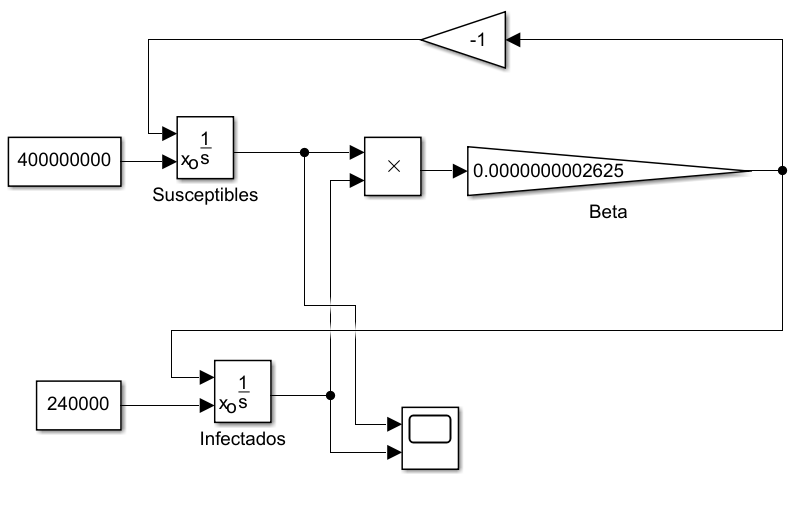
\includegraphics[width=0.9\textwidth]{img/modelo_SI.png}
        \caption{Diagrama de bloques en Simulink para el modelo SI.}
        \label{fig: diagrama de bloques en Simulink para el modelo SI}
        
\end{figure}

\textbf{Modelo SIS} representado en la figura \ref{fig: diagrama de bloques en Simulink para el modelo SIS}, contempla que los individuos infectados pueden recuperarse pero sin adquirir inmunidad, volviendo al estado susceptible.
\begin{figure}[H]
        \centering
        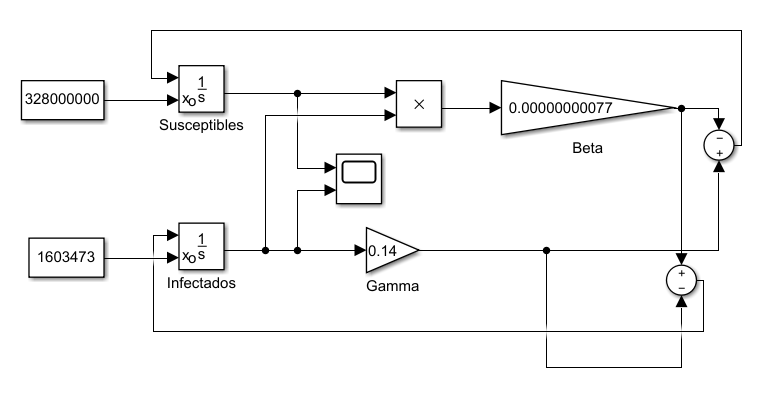
\includegraphics[width=0.9\textwidth]{img/modelo_SIS.png}
        \caption{Diagrama de bloques en Simulink para el modelo SIS.}
        \label{fig: diagrama de bloques en Simulink para el modelo SIS}
        
\end{figure}

\textbf{Modelo SIR} representado en la figura \ref{fig: diagrama de bloques en Simulink para el modelo SIR}, los individuos susceptibles pueden infectarse, pasar a infectados y posteriormente recuperarse con inmunidad permanente.


\begin{figure}[H]
        \centering
        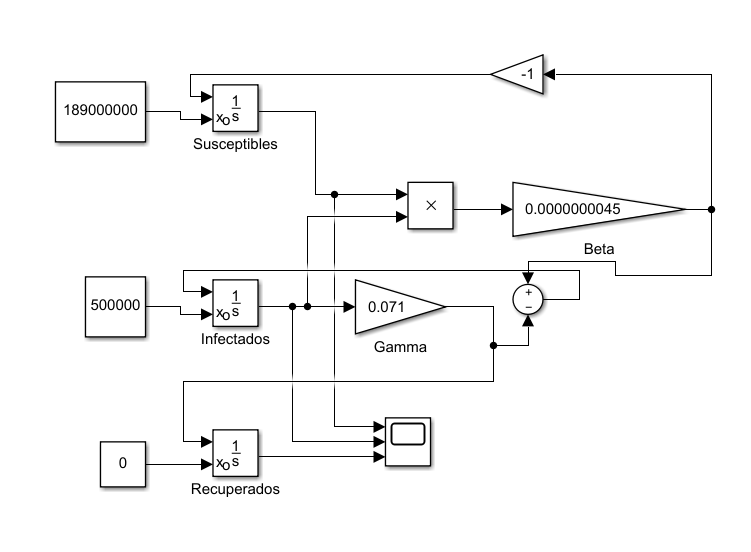
\includegraphics[width=0.9\textwidth]{img/modelo_SIR.png}
        \caption{Diagrama de bloques en Simulink para el modelo SIR.}
        \label{fig: diagrama de bloques en Simulink para el modelo SIR}
        
\end{figure}


\textbf{Modelo SIR con regulador PID} representado en la figura \ref{fig: diagrama de bloques en Simulink para el modelo SIR con regulador PID} corresponde a una extensión del modelo SIR clásico en la que se incorpora un controlador PID. Este regulador actúa sobre la tasa de transmisión con el objetivo de mantener la proporción de individuos infectados por debajo de un valor de referencia, simulando medidas de control sanitario como confinamientos, campañas de vacunación o restricciones de movilidad. El sistema ajusta dinámicamente la intensidad de dichas medidas en función del error entre el número de infectados reales y el deseado, permitiendo evaluar la efectividad de estrategias de intervención automática en la evolución de la epidemia.
\begin{figure}[H]
        \centering
        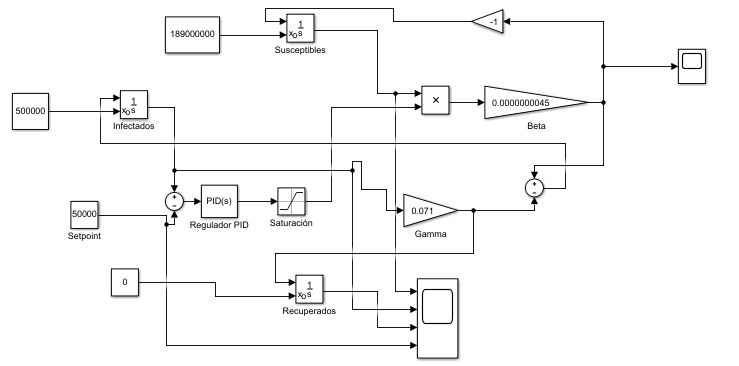
\includegraphics[width=0.9\textwidth]{img/modelo SIR con PID.png}
        \caption{Diagrama de bloques en Simulink para el modelo SIR con regulador PID.}
        \label{fig: diagrama de bloques en Simulink para el modelo SIR con regulador PID}
        
\end{figure}



\textbf{Modelo SEIR} representado en la figura \ref{fig: diagrama de bloques en Simulink para el modelo SEIR}, extensión del modelo SIR que incluye una fase de exposición, donde los individuos están infectados pero no son contagiosos durante un período de incubación.
\begin{figure}[H]
        \centering
        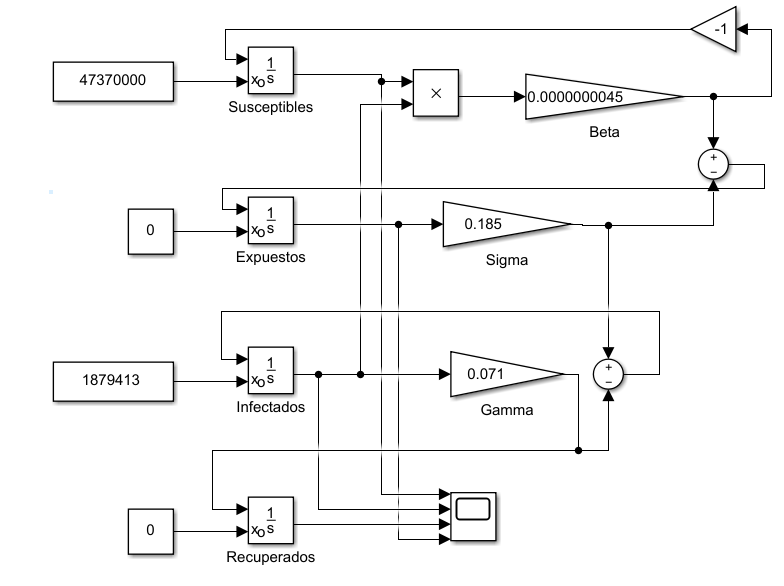
\includegraphics[width=0.9\textwidth]{img/modelo_SEIR.png}
        \caption{Diagrama de bloques en Simulink para el modelo SEIR.}
        \label{fig: diagrama de bloques en Simulink para el modelo SEIR}
        
\end{figure}

\textbf{Modelo SIRV} representado en la figura \ref{fig: diagrama de bloques en Simulink para el modelo SIRV}, modelo SIR que incorpora la vacunación como una vía adicional para pasar de susceptibles a inmunes sin pasar por la infección.
\begin{figure}[H]
        \centering
        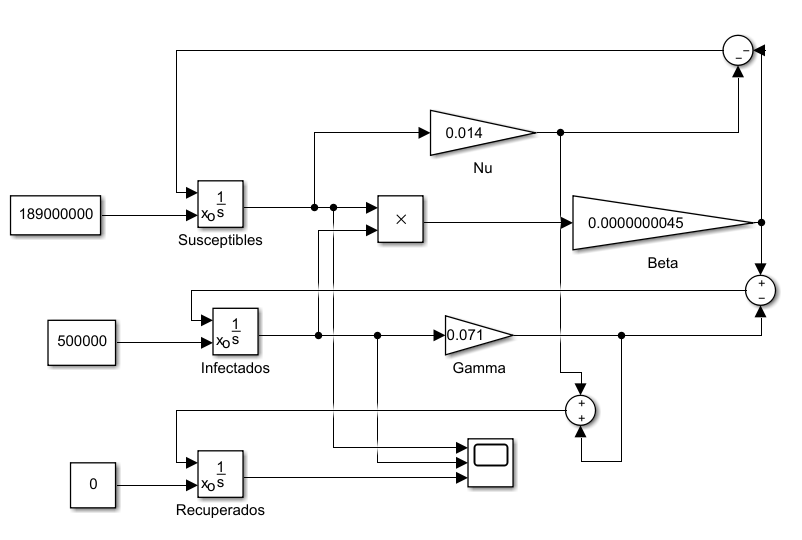
\includegraphics[width=0.9\textwidth]{img/modelo_SIRV_inicio.png}
        \caption{Diagrama de bloques en Simulink para el modelo SIRV.}
        \label{fig: diagrama de bloques en Simulink para el modelo SIRV}
        
\end{figure}


\textbf{Modelo SEIRV} representado en la figura \ref{fig: diagrama de bloques en Simulink para el modelo SEIRV}, modelo SEIR que añade un compartimento para vacunados, permitiendo estudiar el impacto de la vacunación en la dinámica de la epidemia.
\begin{figure}[H]
        \centering
        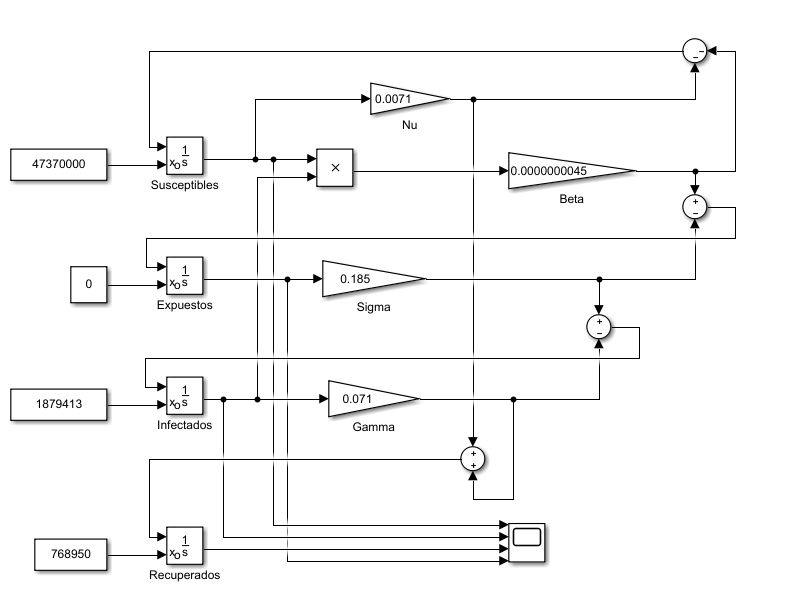
\includegraphics[width=0.9\textwidth]{img/modelo_SEIRV.png}
        \caption{Diagrama de bloques en Simulink para el modelo SEIRV.}
        \label{fig: diagrama de bloques en Simulink para el modelo SEIRV}
       
\end{figure}


\section{Diseño arquitectónico}
El sistema desarrollado consta de tres componentes principales:

\begin{itemize}
    \item \textbf{Modelos en Simulink:} cada modelo epidemiológico se implementa mediante diagramas de bloques que representan las ecuaciones diferenciales del sistema. Esto permite simular la dinámica de la epidemia de manera visual e intuitiva.

    \item \textbf{Scripts en MATLAB:} se utiliza para la implementación del controlador PID en el modelo SIR, actuando sobre la tasa de transmisión para mitigar la propagación.

    \item \textbf{Interfaz gráfica en App Designer:} diseñada para permitir al usuario modificar parámetros epidemiológicos y del controlador, ejecutar simulaciones y visualizar resultados de forma interactiva mediante gráficas dinámicas.
\end{itemize}



En cunato a la aplicación ha sido desarrollada en MATLAB App Designer, lo que proporciona una arquitectura de programación basada en eventos y de programación declarativa para la interfaz de usuario, donde la interfaz gráfica y la lógica de control están encapsuladas en un único archivo `.mlapp'.

El diseño se estructura en los siguientes componentes principales:

\begin{itemize}
    \item \textbf{Interfaz de usuario (UI):} compuesta por elementos gráficos como botones, menús desplegables, campos de entrada numérica y ejes para visualización. Permite al usuario seleccionar el modelo epidemiológico, definir los parámetros iniciales, ejecutar la simulación y visualizar los resultados.
    
    \item \textbf{Controladores (callbacks):} funciones asociadas a eventos de la interfaz gráfica, tales como la selección del modelo o la pulsación del botón de simulación. Estas gestionan la lógica de interacción entre la UI y el núcleo del programa.
    
    \item \textbf{Módulo de simulación:} implementado mediante funciones anónimas de MATLAB y el solucionador \texttt{ode45}, permite resolver los distintos modelos epidemiológicos (SI, SIS, SIR, SEIR, SIRV, SEIRV) a partir de los parámetros definidos por el usuario.
    
    \item \textbf{Visualización de resultados:} Utiliza la función \texttt{plot} para representar la evolución temporal de las variables del modelo. Las leyendas y los ejes se ajustan dinámicamente según el modelo seleccionado.
\end{itemize}


\textbf{Diagrama de clases}.
La clase principal aplicacion\_modelos agrupa todos los elementos de la interfaz de usuario (UI), así como las funciones necesarias para gestionar eventos y simular los modelos epidemiológicos. Se emplea un enfoque orientado a eventos, donde la lógica de simulación se encuentra encapsulada en funciones de devolución de llamada (callbacks). El diagrama de clases se puede ver en la figura \ref{fig: diagrama de clases de la aplicación realizada.}.

\begin{figure}[H]
        \centering
        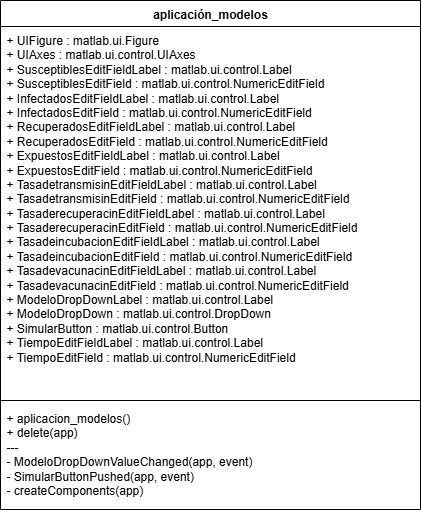
\includegraphics[width=0.9\textwidth]{img/Diagrama sin título.drawio.png}
        \caption{Diagrama de clases de la aplicación realizada.}
        \label{fig: diagrama de clases de la aplicación realizada.}   
\end{figure}









\apendice{Especificación de Requisitos}
\section{Diagrama de casos de uso}


En la Figura~\ref{fig: casos de uso} se presenta el diagrama de casos de uso de la aplicación realizada, en el que se describen las distintas interacciones que pueden realizar los usuarios, dependiendo de si tienen MATLAB instalado o no.

\begin{itemize}
    \item El \textbf{usuario con MATLAB} puede abrir directamente la aplicación desde el archivo \texttt{.mlapp}, seleccionar el modelo epidemiológico, introducir los parámetros, ejecutar la simulación y visualizar los resultados, también se puede simular desdpués de elegir el modelo ya que .
    
    \item El \textbf{usuario sin MATLAB} debe primero instalar los \textit{MATLAB Runtimes} mediante el instalador \texttt{myAppInstaller\_web.exe}, y posteriormente ejecutar la aplicación compilada \texttt{.exe}. Una vez completados estos pasos, podrá seguir el mismo flujo funcional que el usuario con MATLAB.
    
    \item Los casos de uso principales compartidos por ambos tipos de usuario son: \textit{Seleccionar modelo}, \textit{Introducir parámetros}, \textit{Simular} y \textit{Visualización de resultados}.
\end{itemize}

\begin{figure}[H]
        \centering
        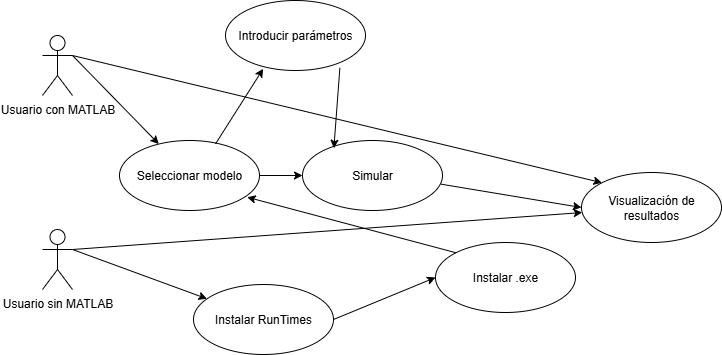
\includegraphics[width=0.9\textwidth]{img/diagrama casos.drawio.png}
        \caption{Diagrama de casos de uso de la aplicación realizada.}
        \label{fig: casos de uso}
        
\end{figure}


\section{Explicación casos de uso}
A continuación en las diferentes tablas (\ref{tab:cu1})(\ref{tab:cu2})(\ref{tab:cu3})(\ref{tab:cu4})(\ref{tab:cu5})(\ref{tab:cu6}) se detalla la explicación de los casos de usos utilizados en el diagraama de casos de uso del apartado anterior.
\begin{table}[H]
\centering
\begin{tabular}{|p{3cm}|p{9cm}|}
\hline
\textbf{CU-1} & \textbf{Seleccionar modelo} \\
\hline
\textbf{Versión} & 1.0 \\
\hline
\textbf{Autor} & Lucía Segura Benito \\
\hline
\textbf{Requisitos asociados} & RF-01 \\
\hline
\textbf{Descripción} & El usuario selecciona el tipo de modelo epidemiológico a utilizar: SI, SIS, SIR, SEIR, SIRV o SEIRV. \\
\hline
\textbf{Precondición} & La aplicación debe estar abierta. \\
\hline
\textbf{Acciones} &
\begin{enumerate}
    \item El usuario abre el menú desplegable de modelos.
    \item Selecciona uno de los modelos disponibles.
    \item El sistema guarda la selección para la simulación posterior.
\end{enumerate}
\\
\hline
\textbf{Postcondición} & Modelo seleccionado queda registrado en la aplicación. \\
\hline
\textbf{Excepciones} & No se produce ninguna si el desplegable está bien cargado. \\
\hline
\textbf{Importancia} & Alta \\
\hline
\end{tabular}
\caption{CU-1: Seleccionar modelo.}
\label{tab:cu1}
\end{table}



\begin{table}[H]
\centering
\begin{tabular}{|p{3cm}|p{9cm}|}
\hline
\textbf{CU-2} & \textbf{Introducir parámetros} \\
\hline
\textbf{Versión} & 1.0 \\
\hline
\textbf{Autor} & Lucía Segura Benito \\
\hline
\textbf{Requisitos asociados} & RF-02 \\
\hline
\textbf{Descripción} & El usuario introduce los valores numéricos requeridos para simular el modelo seleccionado. \\
\hline
\textbf{Precondición} & Un modelo debe estar previamente seleccionado. \\
\hline
\textbf{Acciones} &
\begin{enumerate}
    \item El usuario accede a los campos de parámetros.
    \item Introduce valores que se piden dependiendo del modelo seleccionado.
    \item El sistema almacena los parámetros para usarlos en la simulación.
\end{enumerate}
\\
\hline
\textbf{Postcondición} & Parámetros definidos correctamente para la simulación. \\
\hline
\textbf{Excepciones} & Parámetros vacíos o no válidos (el sistema muestra mensaje de error). \\
\hline
\textbf{Importancia} & Alta \\
\hline
\end{tabular}
\caption{CU-2: Introducir parámetros.}
\label{tab:cu2}
\end{table}






\begin{table}[H]
\centering
\begin{tabular}{|p{3cm}|p{9cm}|}
\hline
\textbf{CU-3} & \textbf{Simular modelo} \\
\hline
\textbf{Versión} & 1.0 \\
\hline
\textbf{Autor} & Lucía Segura Benito \\
\hline
\textbf{Requisitos asociados} & RF-03, RF-04 \\
\hline
\textbf{Descripción} & El usuario ejecuta la simulación del modelo epidemiológico seleccionado utilizando los parámetros introducidos. \\
\hline
\textbf{Precondición} & El modelo debe estar seleccionado y los parámetros correctamente definidos. \\
\hline
\textbf{Acciones} &
\begin{enumerate}
    \item El usuario pulsa el botón "Simular".
    \item El sistema verifica que los datos de entrada sean válidos.
    \item El sistema ejecuta el modelo epidemiológico seleccionado.
    \item Se muestran los resultados en pantalla mediante gráficas.
\end{enumerate}
\\
\hline
\textbf{Postcondición} & Los resultados de la simulación se visualizan en la interfaz de usuario. \\
\hline
\textbf{Excepciones} & Parámetros incompletos o inválidos (el sistema muestra un mensaje de error). \\
\hline
\textbf{Importancia} & Alta \\
\hline
\end{tabular}
\caption{CU-3: Simular modelo.}
\label{tab:cu3}
\end{table}



\begin{table}[H]
\centering
\begin{tabular}{|p{3cm}|p{9cm}|}
\hline
\textbf{CU-4} & \textbf{Visualización de resultados} \\
\hline
\textbf{Versión} & 1.0 \\
\hline
\textbf{Autor} & Lucía Segura Benito \\
\hline
\textbf{Requisitos asociados} & RF-05 \\
\hline
\textbf{Descripción} & La aplicación muestra al usuario los resultados de la simulación mediante gráficos. \\
\hline
\textbf{Precondición} & Simulación completada exitosamente. \\
\hline
\textbf{Acciones} &
\begin{enumerate}
    \item El sistema genera gráficos de las variables.
    \item Los gráficos se muestran en la interfaz.
\end{enumerate}
\\
\hline
\textbf{Postcondición} & Gráficas epidemiológicas visibles para el usuario. \\
\hline
\textbf{Excepciones} & Error al renderizar gráficos (muy raro). \\
\hline
\textbf{Importancia} & Media \\
\hline
\end{tabular}
\caption{CU-4: Visualización de resultados.}
\label{tab:cu4}
\end{table}




\begin{table}[H]
\centering
\begin{tabular}{|p{3cm}|p{9cm}|}
\hline
\textbf{CU-5} & \textbf{Instalar RunTimes} \\
\hline
\textbf{Versión} & 1.0 \\
\hline
\textbf{Autor} & Lucía Segura Benito \\
\hline
\textbf{Requisitos asociados} & RF-06 \\
\hline
\textbf{Descripción} & El usuario sin MATLAB instala los MATLAB Runtime necesarios para ejecutar la aplicación compilada. \\
\hline
\textbf{Precondición} & No disponer de MATLAB instalado. Tener el archivo \texttt{myAppInstaller\_web.exe}. \\
\hline
\textbf{Acciones} &
\begin{enumerate}
    \item El usuario ejecuta el archivo \texttt{myAppInstaller\_web.exe}.
    \item El instalador descarga e instala los runtimes de MATLAB (MCR).
\end{enumerate}
\\
\hline
\textbf{Postcondición} & Los runtimes de MATLAB quedan correctamente instalados. \\
\hline
\textbf{Excepciones} & Error en la instalación por permisos, red o espacio en disco. \\
\hline
\textbf{Importancia} & Alta \\
\hline
\end{tabular}
\caption{CU-5: Instalar RunTimes.}
\label{tab:cu5}
\end{table}




\begin{table}[H]
\centering
\begin{tabular}{|p{3cm}|p{9cm}|}
\hline
\textbf{CU-6} & \textbf{Instalar .exe} \\
\hline
\textbf{Versión} & 1.0 \\
\hline
\textbf{Autor} & Lucía Segura Benito \\
\hline
\textbf{Requisitos asociados} & RF-07 \\
\hline
\textbf{Descripción} & El usuario sin MATLAB ejecuta el archivo compilado de la aplicación tras instalar los runtimes. \\
\hline
\textbf{Precondición} & MATLAB Runtime (MCR) instalado previamente. \\
\hline
\textbf{Acciones} &
\begin{enumerate}
    \item El usuario ejecuta \texttt{aplicacion\_modelos.exe}.
    \item Se lanza la aplicación de forma autónoma, sin requerir MATLAB.
\end{enumerate}
\\
\hline
\textbf{Postcondición} & Aplicación ejecutándose de forma normal. \\
\hline
\textbf{Excepciones} & Error al lanzar el .exe, falta de runtimes o permisos insuficientes. \\
\hline
\textbf{Importancia} & Alta \\
\hline
\end{tabular}
\caption{CU-6: Instalar .exe.}
\label{tab:cu6}
\end{table}

\apendice{Estudio experimental}
\apendice{Anexo de sostenibilidad curricular}

Este proyecto está centrado en el modelado matemático de epidemias mediante modelos compartimentales y su implementación en \texttt{MATLAB} y \texttt{Simulink}, se vincula de forma directa con diversos ODS\footnote{Objetivos de Desarrollo Sostenible} establecidos en la Agenda 2030 de las Naciones Unidas \cite{onu2015agenda2030}.

\section*{ODS relacionados}

\begin{itemize}
    \item \textbf{ODS 3: Salud y Bienestar.} El proyecto contribuye al entendimiento de la propagación de enfermedades infecciosas y la evaluación de estrategias de control como la vacunación y las cuarentenas, aspectos clave para mejorar la resiliencia de los sistemas sanitarios ante futuras pandemias \cite{who2020disorder}.
    
    \item \textbf{ODS 4: Educación de Calidad.} La creación de una aplicación interactiva para la visualización y manipulación de los modelos permite democratizar el acceso al conocimiento técnico, facilitando la comprensión de dinámicas epidemiológicas incluso a personas sin formación especializada. Esto potencia el aprendizaje autónomo y el desarrollo de competencias digitales \cite{unesco2020education}.
    
    \item \textbf{ODS 10: Reducción de las Desigualdades.} Al permitir la simulación y análisis de medidas sanitarias en distintos escenarios, el trabajo también reflexiona sobre cómo las epidemias afectan de manera desigual a distintas poblaciones. El desarrollo de herramientas accesibles y adaptables puede contribuir a reducir brechas tecnológicas y de conocimiento \cite{who2021inequality}.
\end{itemize}

\section*{Contribuciones a la sostenibilidad curricular}

El trabajo fomenta diversas competencias clave para el desarrollo sostenible, alineadas con los principios de la sostenibilidad curricular en educación superior \cite{lozano2017teaching}. Entre ellas destacan:

\begin{itemize}
    \item \textbf{Pensamiento crítico y sistémico:} al modelar fenómenos complejos como la dinámica epidémica desde un enfoque cuantitativo e interdisciplinar.
    \item \textbf{Innovación responsable:} mediante el diseño de herramientas digitales orientadas a la educación y la toma de decisiones en salud pública.
    \item \textbf{Conciencia ética y social:} al abordar la dimensión humana y desigual de las pandemias, así como la necesidad de respuestas colaborativas y equitativas.
\end{itemize}

En conjunto, este trabajo de fin de grado no solo aporta un enfoque técnico y analítico al estudio de epidemias, sino que también contribuye a una visión integral de la sostenibilidad, reconociendo la interdependencia entre ciencia, tecnología, salud pública y justicia social.
De este modo, el TFG se alinea con los principios de una educación superior comprometida con la Agenda 2030 y con la formación de profesionales capaces de abordar los desafíos globales desde una perspectiva ética y sostenible.






\bibliographystyle{apalike}
\bibliography{bibliografiaAnexos}

\end{document}


